\section{Basics}

\subsection[Control Theory]{Control Theory}
\begin{frame}
\frametitle{What is control theory?}
\begin{block}{}
	\textbf{Control theory} is an interdisciplinary branch of engineering and mathematics that deals with the behavior of dynamical systems with inputs, and how their behavior is modified by feedback. The usual objective of control theory is to design a controller that produces inputs to a plant so its output follows a desired reference signal which may be a fixed or changing value. - \href{https://en.wikipedia.org/wiki/Control_theory}{wikipedia} 
\end{block}
\begin{figure}
	\centering
	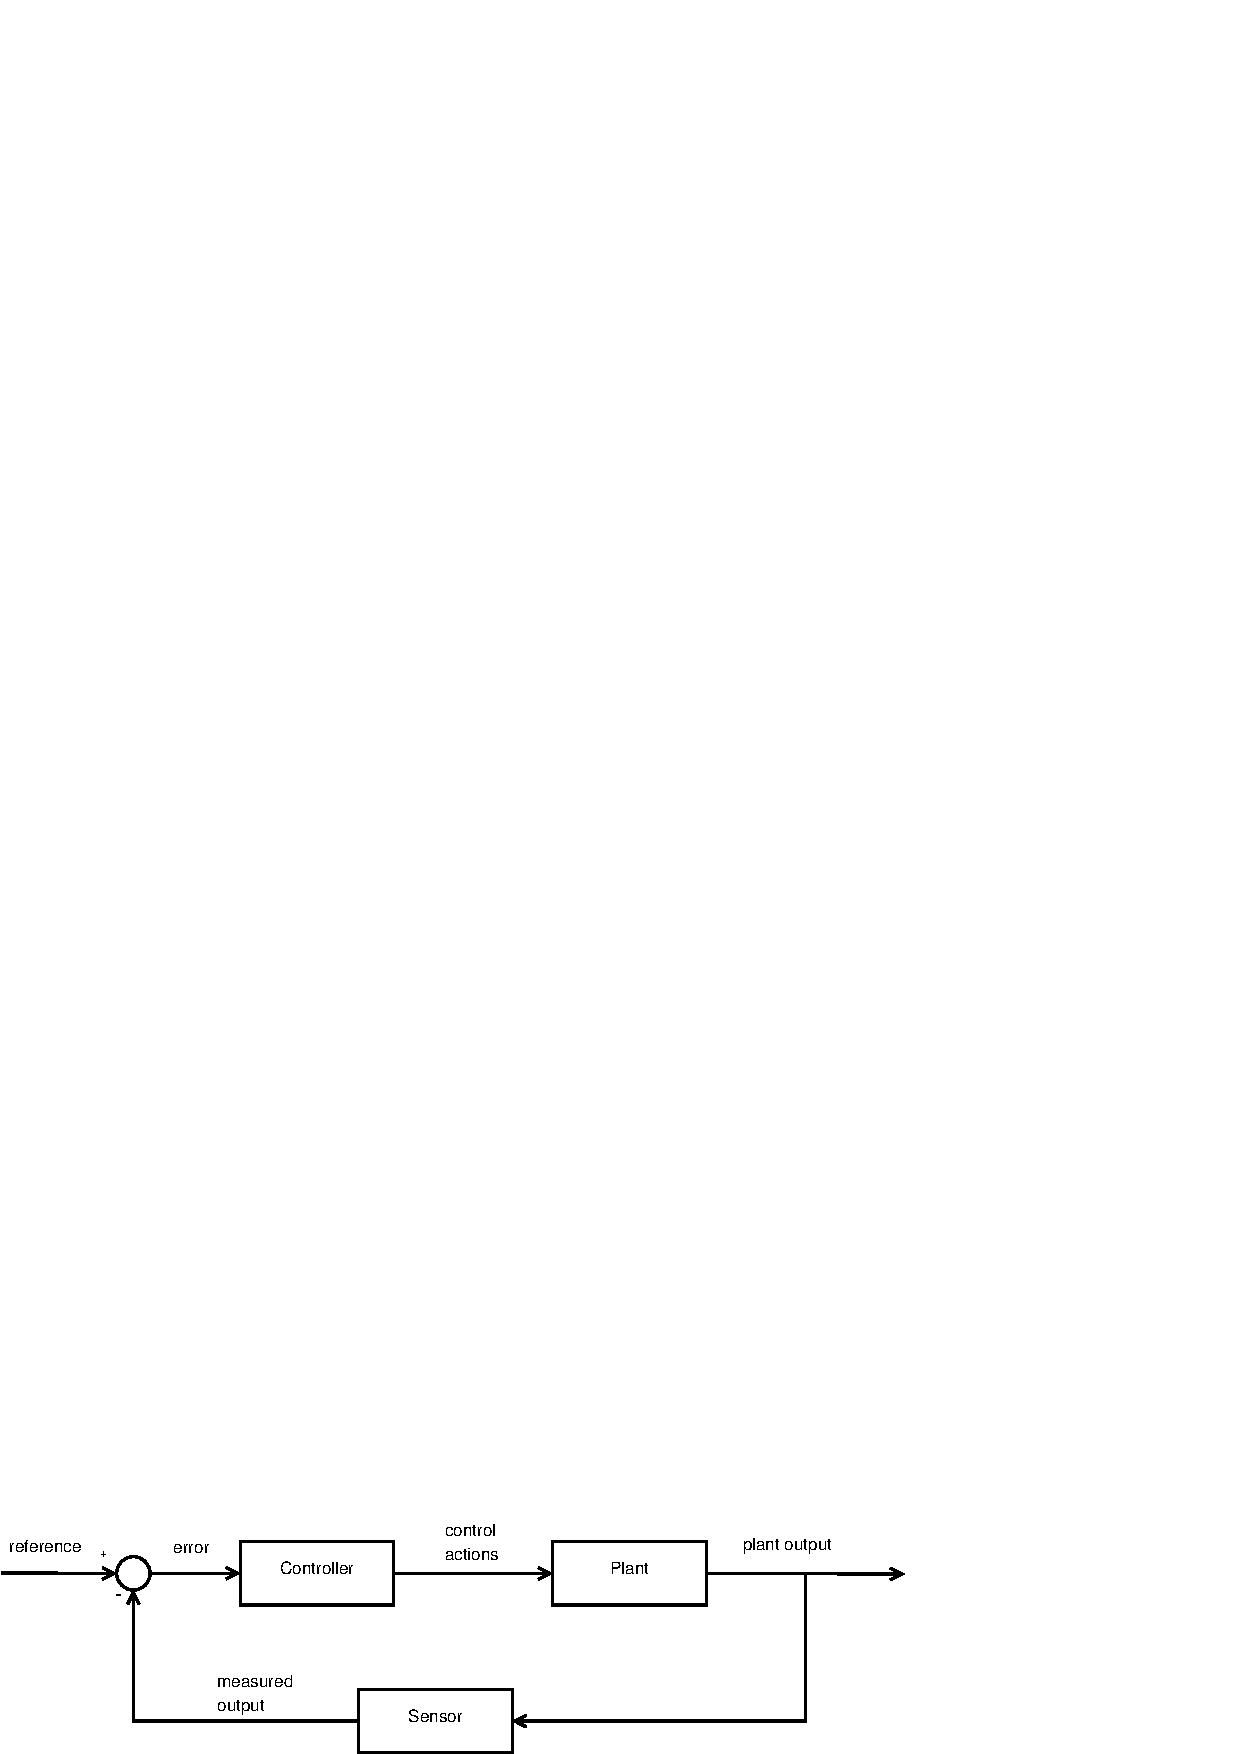
\includegraphics[width=1\linewidth]{controlsystem}
	\label{fig:controlsystem}
\end{figure}
\end{frame}

\begin{frame}
	\frametitle{Controllers}
	\begin{block}{Types of controllers}
		\begin{itemize}
			\item On-off controller
			\begin{itemize}
				\item e.g., Thermostate at home
			\end{itemize}
			\item \textbf{PID controllers, Lead and lag compensators (this course)}
			\begin{itemize}
				\item Cruise-control in your car
				\item Temperature, level, flow, presssure, pH, ... in chemical plants
			\end{itemize}
			\item More advanced controllers
			\begin{itemize}
				\item State-space feedback controllers (e.g., LQR)
				\item Model Predictive Controller (MPC)
				\item Fuzzy Control
				\item Neuro-fuzzy Control
				\item ...
			\end{itemize}
		\end{itemize}
	\end{block}
\end{frame}


\begin{frame}
	\frametitle{Open-loop System}
	\begin{definition}
		In an open loop control system the actual output signal $Y(s)$ has no effect on the control action U(s).
		\vspace{-1em}
		\begin{figure}
			\centering
			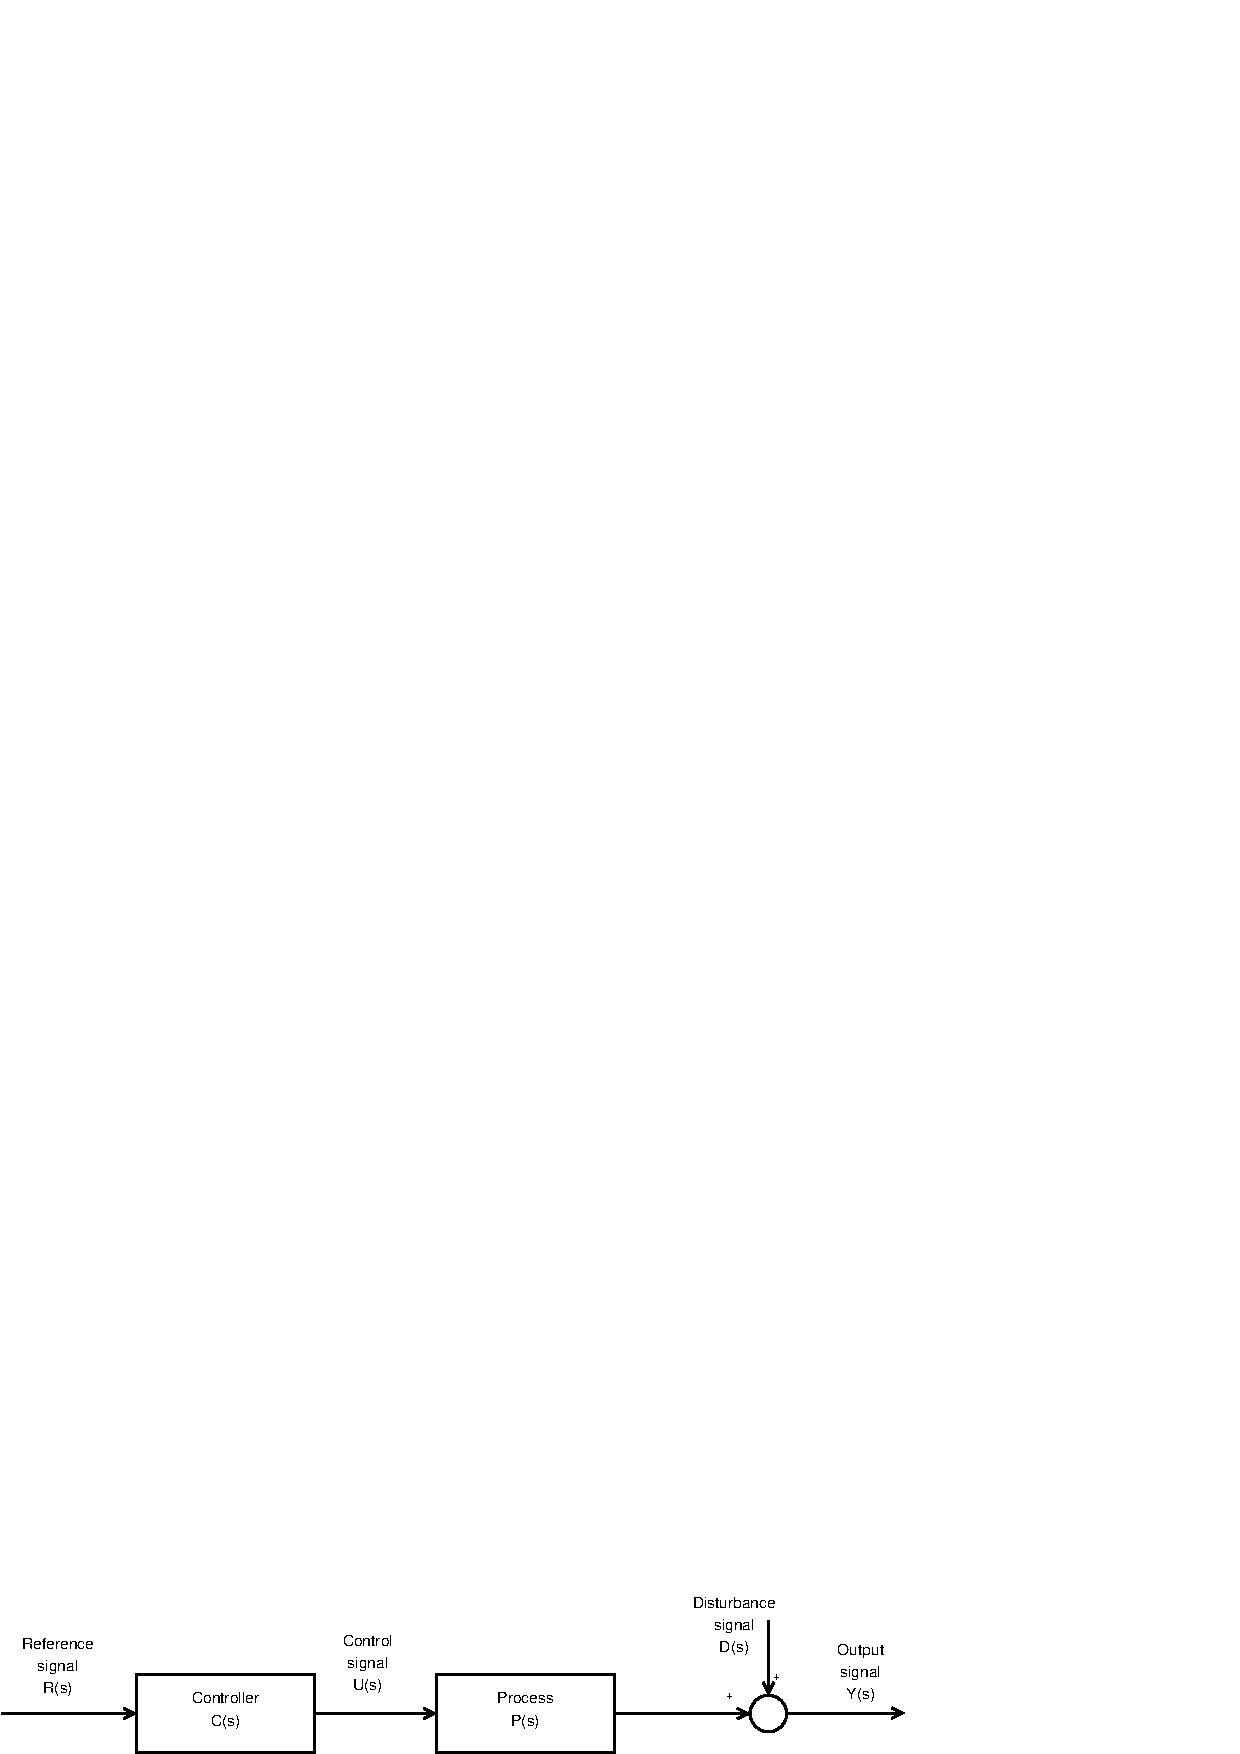
\includegraphics[width=1\linewidth]{Open-Loop}
			\label{fig:Open-Loop}
		\end{figure}
		\begin{align*}
		Y(s) = P(s)U(s) = P(s)C(s)R(s) \\
		\end{align*}
	\end{definition}
\end{frame}

\begin{frame}
	\frametitle{Open-loop System}
	\vspace*{-1em}
	\begin{example}
		\begin{minipage}{0.5\linewidth}
			\begin{itemize}
				\item You are pouring a glass of water, but you \textbf{cannot look at the glass}.
				\item The desired output is a full glass of water within a reasonable time.
				\item The input can have two values: on or off (assume a quite primitive tap).
				\item It will not be easy to do this successfully.
			\end{itemize}
		\end{minipage}
		\hfill
		\begin{minipage}{0.48\linewidth}
			\begin{figure}
				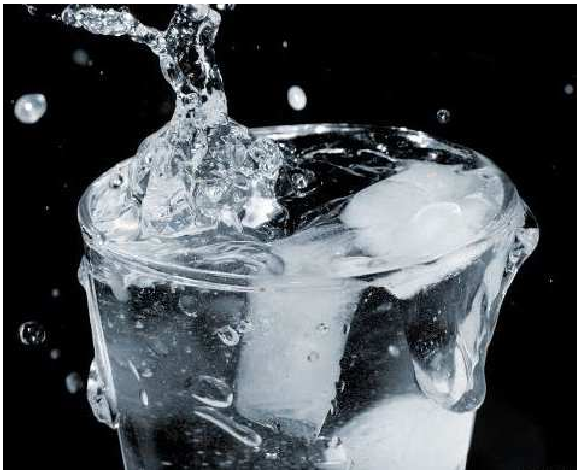
\includegraphics[width=1\linewidth]{glass}
			\end{figure}
		\end{minipage}
		\parbox{\linewidth}{\vspace{1em} \quad The solution is evident: look at the glass while pouring!}
	\end{example}
\end{frame}

\begin{frame}
	\frametitle{Closed-loop system}
	\begin{definition}
		In a closed-loop system the output of the controller is influenced by the output of the system using a \textbf{negative feedback loop}.
	\end{definition}
	\begin{block}{Classical control-loop}
		\begin{figure}
			\centering
			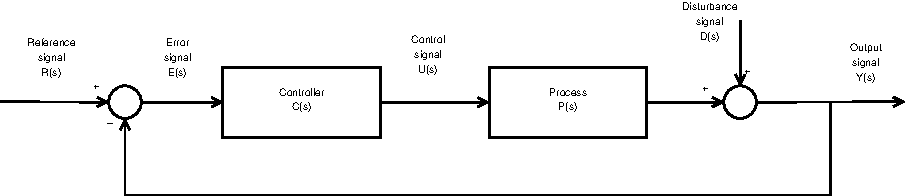
\includegraphics[width=0.9\linewidth]{Closed-Loop}
			\label{fig:Closed-Loop}
		\end{figure}
		\vspace{1em}
		\[ Y(s) =  \frac{P(s)C(s)}{1 + P(s)C(s)}R(s) \text{\quad when D(s) = 0}\]
	\end{block}
\end{frame}


\begin{frame}
	\begin{block}{Digital Control Loop}
		\begin{figure}
			\centering
			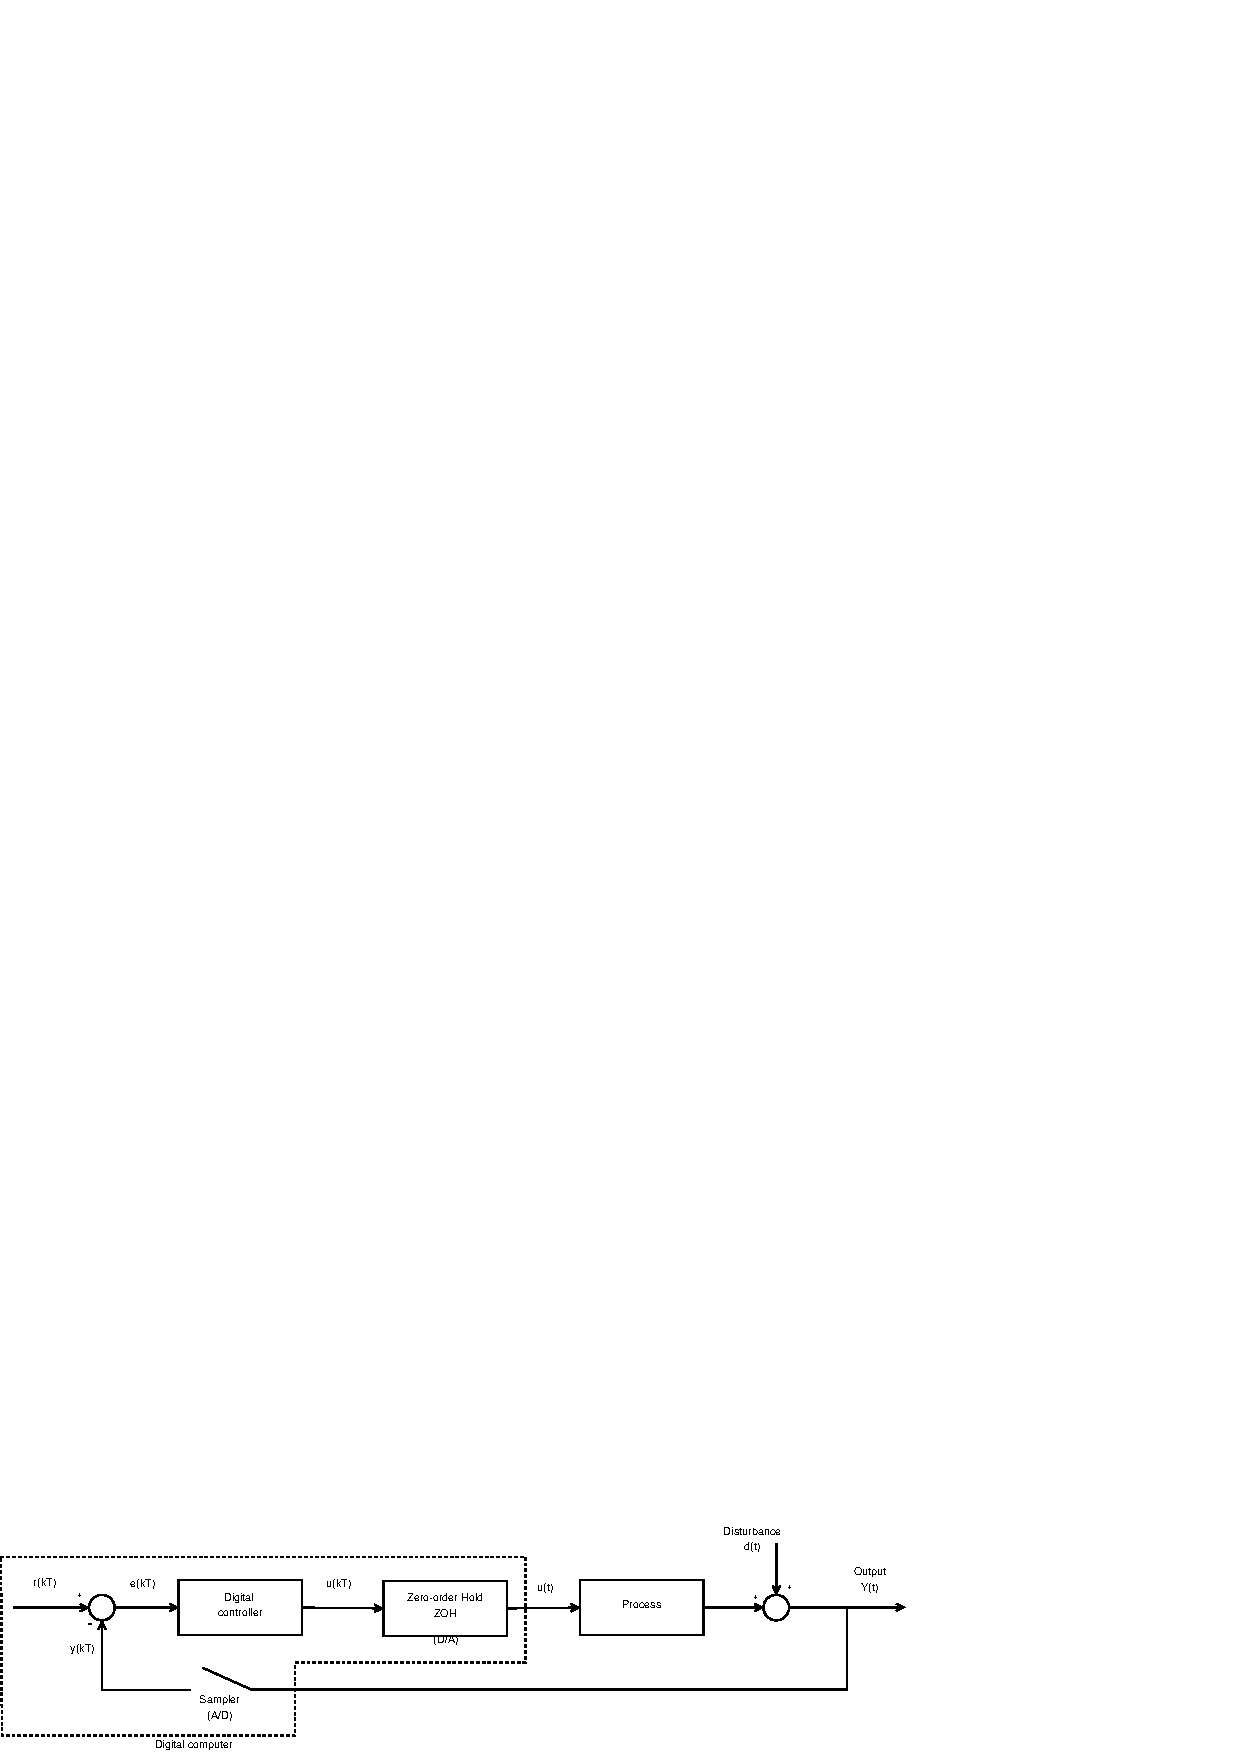
\includegraphics[width=1\linewidth]{digital-control-system}
			\label{fig:digital-control-system}
		\end{figure}
	\end{block}
\end{frame}

\subsection[Demo: Inverted Pendulum]{Demo: Inverted Pendulum}
\begin{frame}
	\begin{figure}
\centering
\href{http://homes.esat.kuleuven.be/~magudelo/_html5/test11.html}{\includegraphics[width=1\linewidth]{"inverted-pendulum/full"}}
\label{fig:InvertedPendulum}
\end{figure}
\end{frame}

\section{Control Goals}
\begin{frame}
	\frametitle{What is good control?}
	\begin{block}{}
		Good control depends on the application
	\end{block}
	\begin{block}{Control Goals}
		\begin{itemize}
			\item Stability
			\item Disturbance rejection
			\item Reference tracking
			\item Robustness
			\item ...
		\end{itemize}
	\end{block}
\end{frame}

\subsection[Examples]{Examples}

\begin{frame}
	\frametitle{Examples: Stability}
\begin{figure}
\centering
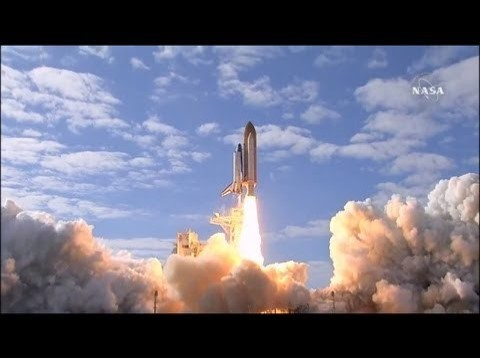
\includegraphics[width=0.6\linewidth]{control-goals/shuttle}
\caption{Space shuttles are like inverted pendulums. Control systems make sure they do not flip over.}
\label{fig:shuttle}
\end{figure}
\end{frame}

\begin{frame}
	\frametitle{Examples: Disturbance rejection}
	\begin{itemize}
		\item Your body will try to keep your internal temperature as constant as possible, no matter how hot/cold it is outside.
	\end{itemize}
	\begin{figure}
		\centering
		\begin{minipage}{0.45\textwidth}
			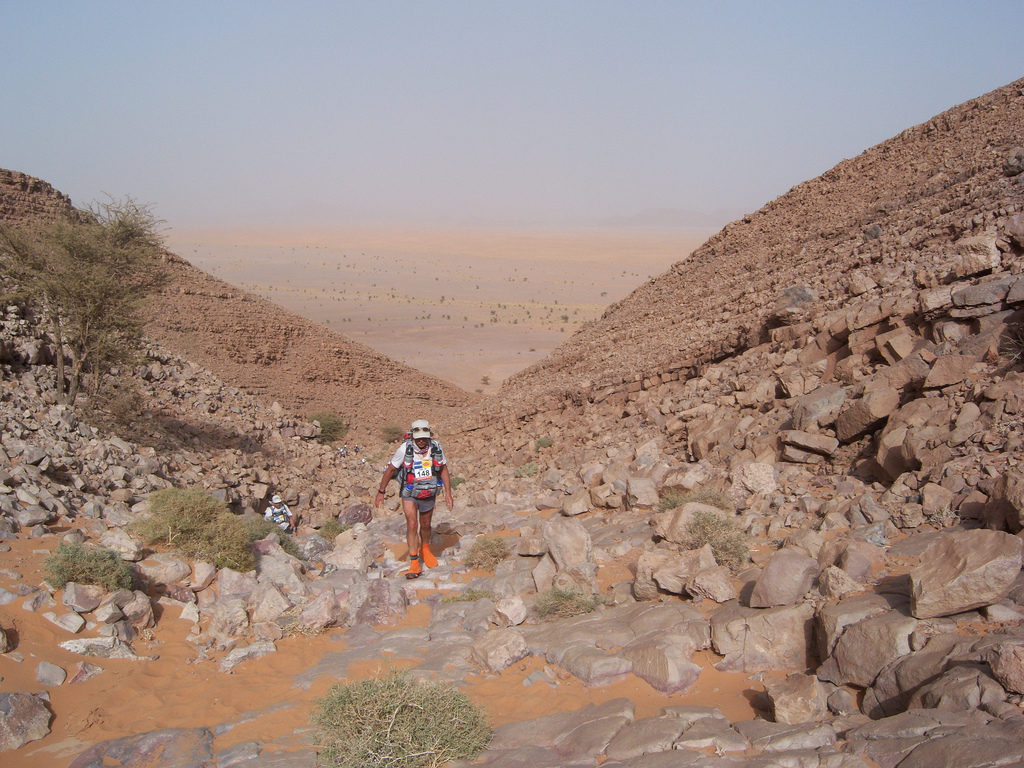
\includegraphics[width=0.7\linewidth]{control-goals/marathon-des-sables}
			\caption{\href{https://www.flickr.com/photos/61680535@N07/5625053385/}{\parbox{\linewidth}{\tiny Flickr.com \\ \underline{tent86} \\ Marathon Des Sables 046}}}
			\label{fig:marathon-des-sables}
		\end{minipage}
		\centering
		\begin{minipage}{0.45\textwidth}
			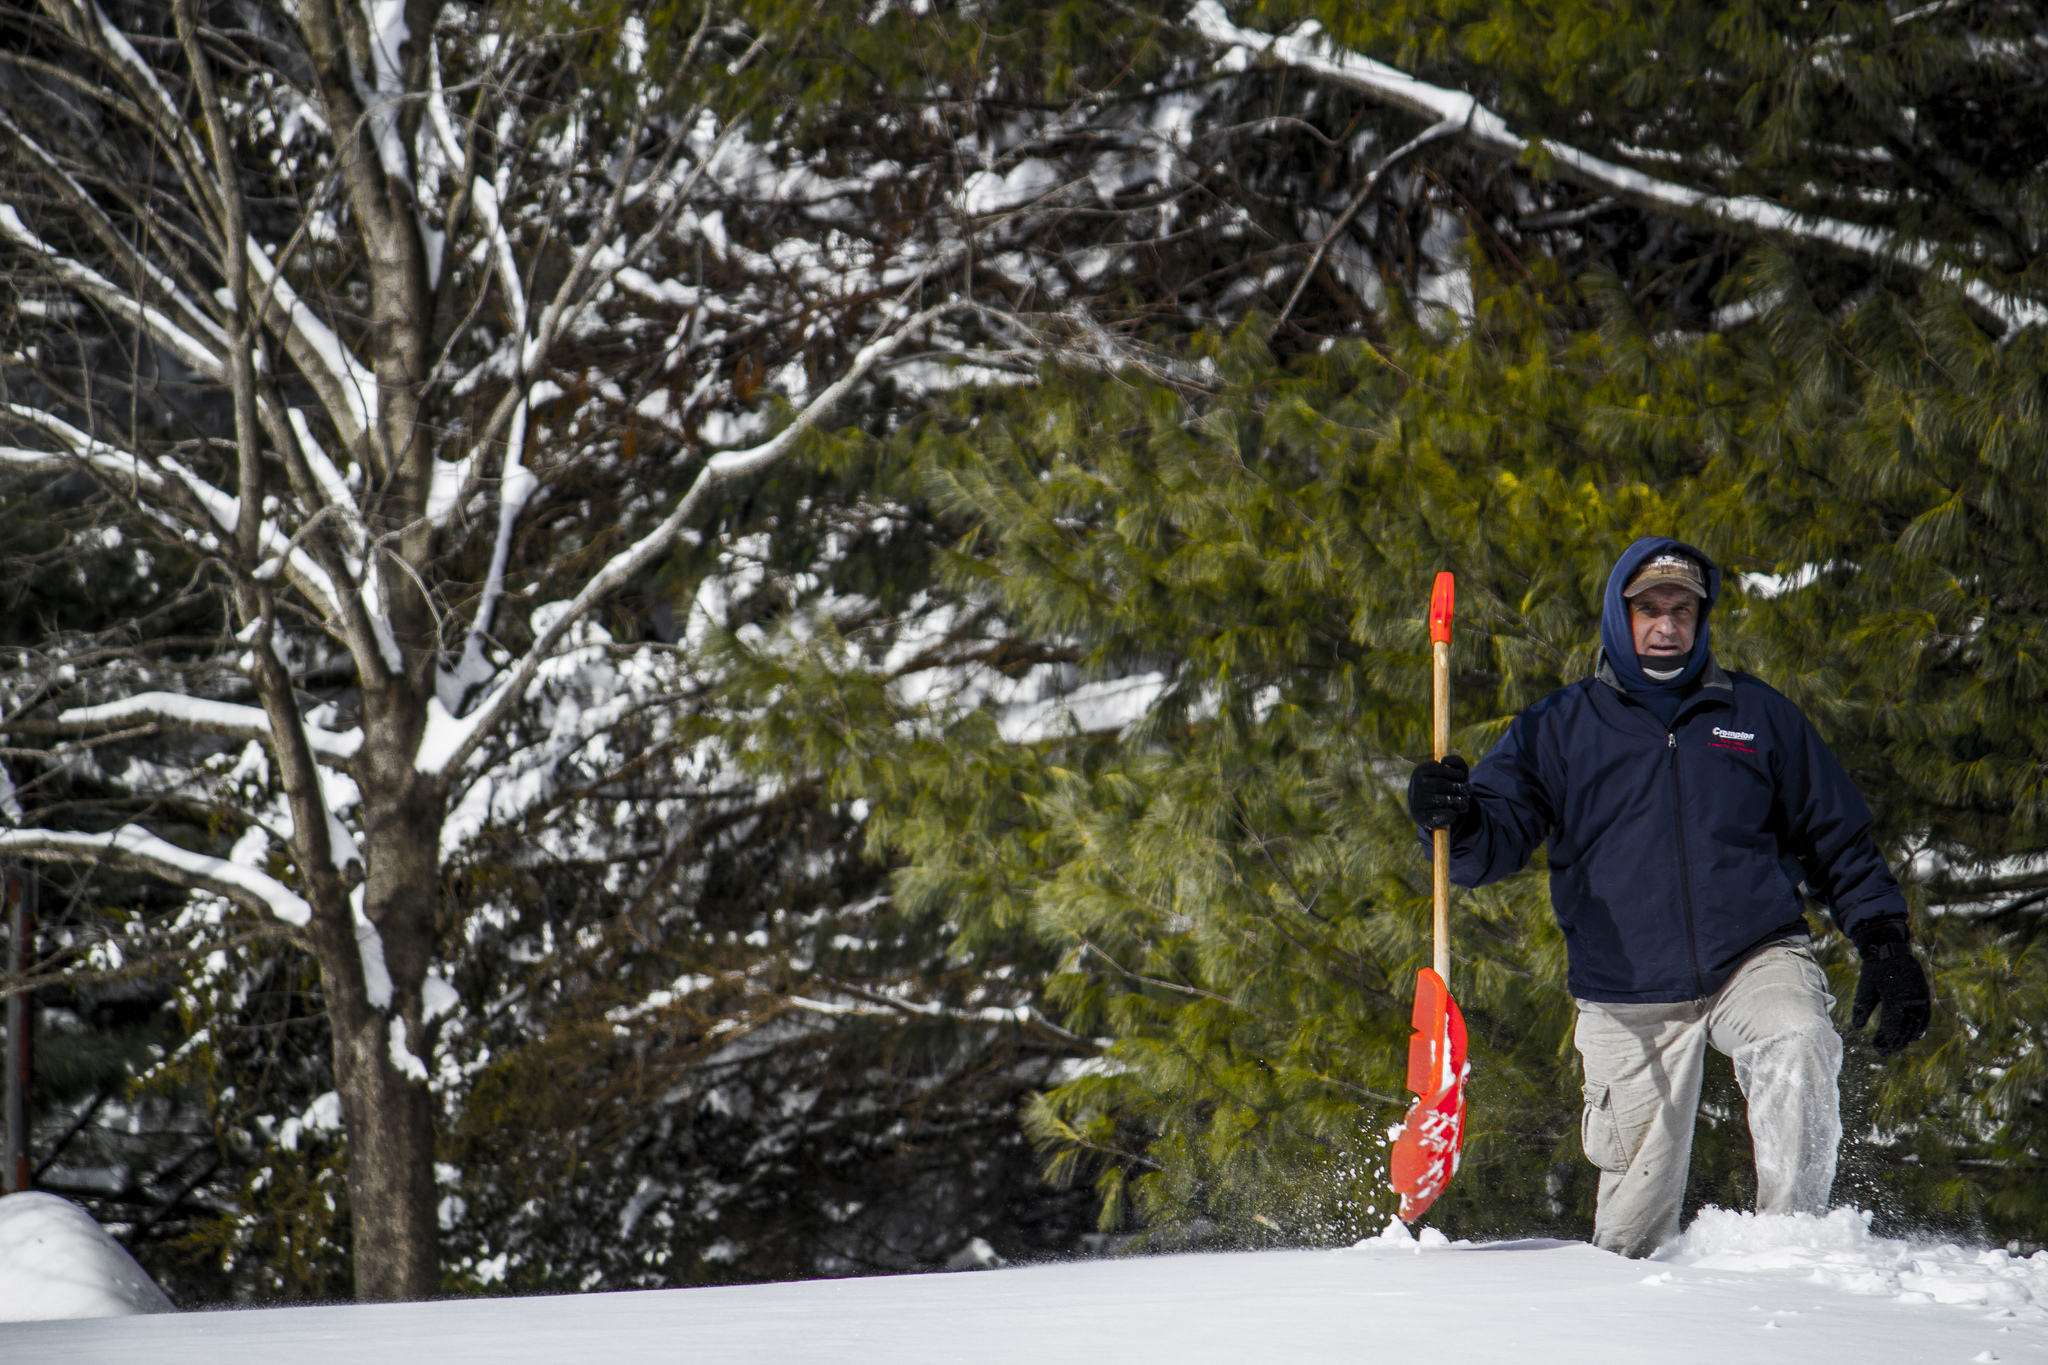
\includegraphics[width=0.8\linewidth]{control-goals/enduring}
			\caption{\parbox{\linewidth}{\tiny \href{https://www.flickr.com/photos/kaiban/8515218404/in/photolist-dYsHLq}{\underline{Jack Zalium} \\ Enduring} \\ \href{https://creativecommons.org/licenses/by-nd/2.0/}{Creative Commons}}}
			\label{fig:enduring}
		\end{minipage}
	\end{figure}
\end{frame}

\begin{frame}
	\frametitle{Examples: Reference tracking}
	\begin{figure}
		\centering
		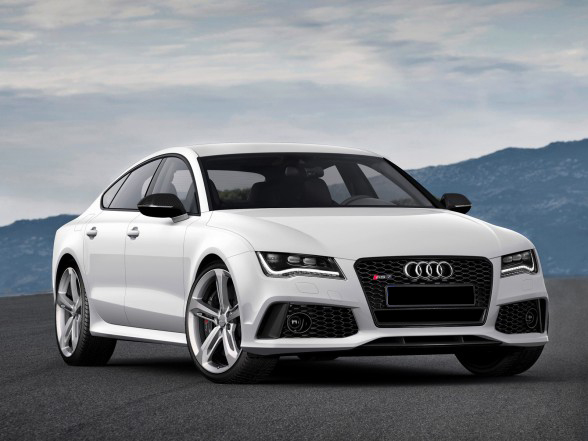
\includegraphics[width=0.6\linewidth]{control-goals/audi}
		\caption{Audi has a system for automatic driving in traffic jams. The audi will follow the car in front at an appropriate distance. \href[pdfnewwindow=true]{https://www.youtube.com/watch?v=Qa_ZSRj0WM0}{\nolinkurl{https://www.youtube.com/watch?v=Qa_ZSRj0WM0}}}
		\label{fig:audi-tracking}
	\end{figure}
\end{frame}


\begin{frame}
	\frametitle{Examples: Robustness}
	\begin{figure}
		\centering
		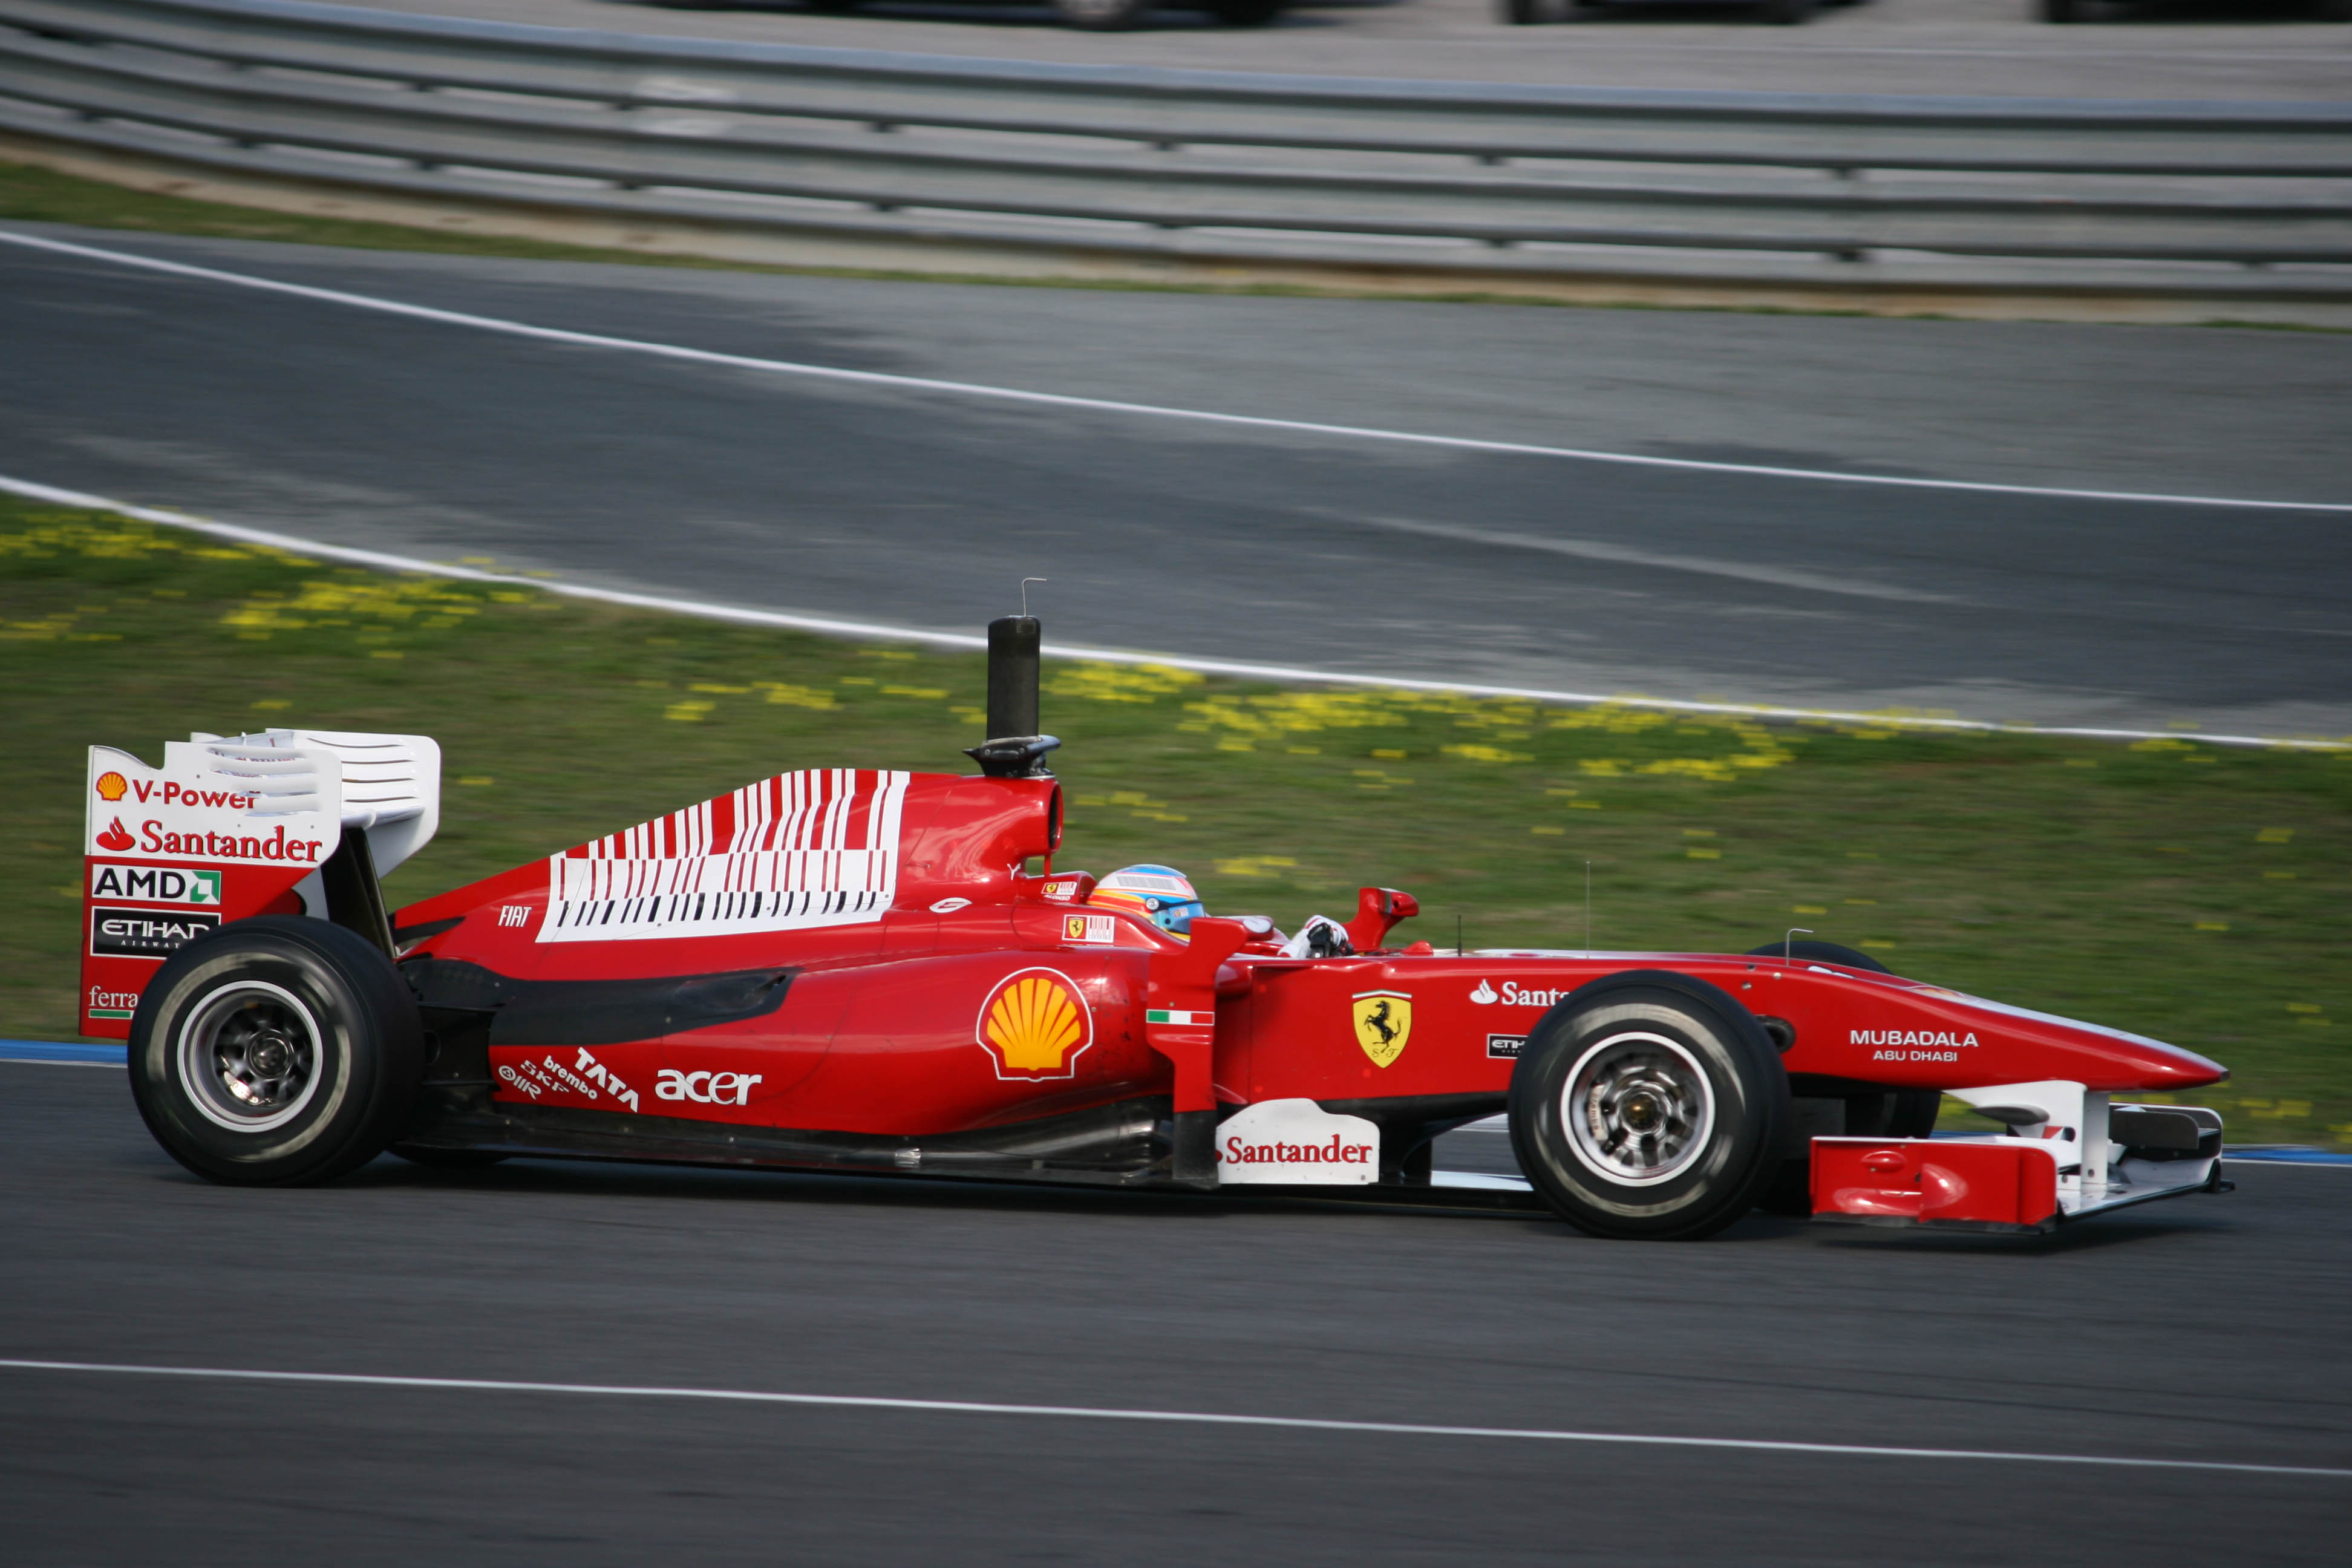
\includegraphics[width=0.7\linewidth]{control-goals/formula-1}
		\caption{It is not possible to drive a formula 1 car using your knowledge of regular cars. However, you can drive a wide variety of road cars.}
		\label{fig:formula-1}
	\end{figure}
\end{frame}

\subsection[Exercise]{Exercise}
\begin{frame}
	\frametitle{Exercise: Could you name the correct property?}
	\begin{figure}
\centering
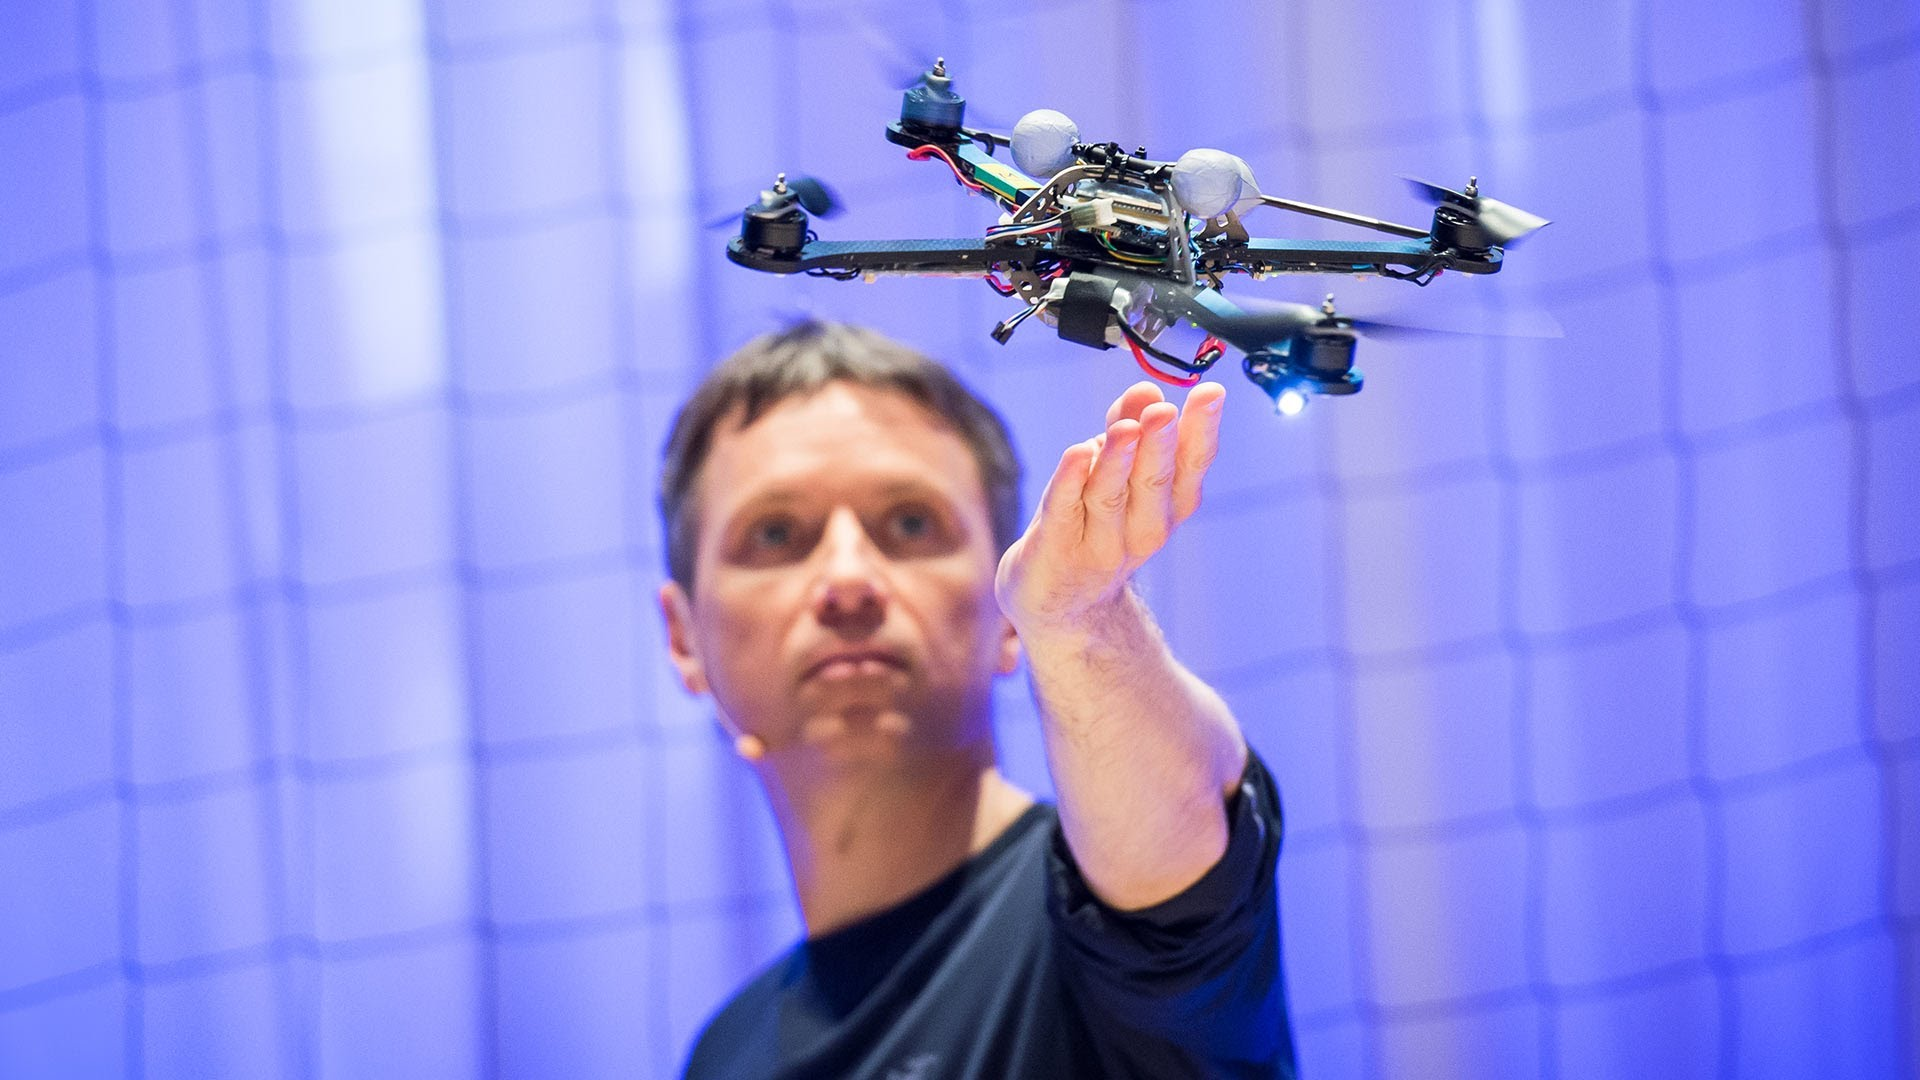
\includegraphics[width=1\linewidth]{control-goals/quadcopter}
\label{fig:ted-drone}
\end{figure}

\end{frame}


\section{Closed-loop systems}
\begin{frame}
	\frametitle{Transfer function of a closed-loop system}
	\begin{block}{Classical control loop}
		\begin{figure}
			\centering
			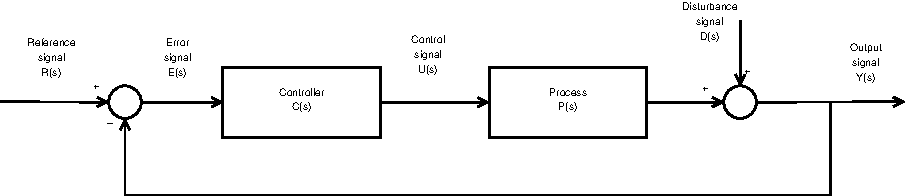
\includegraphics[width=1\linewidth]{Closed-Loop}
			\label{fig:Closed-Loop2}
		\end{figure}
		\vspace{0.2em}
	\end{block}
	\begin{block}{}
		\begin{flalign*}
			Y(s) - D(s) &= P(s)U(s) \quad \text{with } U(s) = C(s)E(s) \\
			Y(s) - D(s) &= P(s)C(s)E(s) \quad \text{with } E(s) = R(s) - Y(s) \\
		\end{flalign*}
	\end{block}
\end{frame}
\begin{frame}
	\begin{block}{}
		\begin{flalign*}
			Y(s) - D(s) &= P(s)C(s) (R(s) - Y(s)) \\
			Y(s) - D(s) &= P(s)C(s)R(s) - P(s)C(s)Y(s) \\
		\end{flalign*}
	\end{block}
	\begin{alertblock}{}
		\[
			Y(s) = \frac{P(s)C(s)}{1 + P(s)C(s)}R(s) + \frac{1}{1 + P(s)C(s)}D(s)
		\]
	\end{alertblock}
\end{frame}


\begin{frame}
	\frametitle{Transfer function from $R(s)$ to $Y(s)$}
	\begin{definition}
		We define $H(s)$ as the transfer function from $R(s)$ to $Y(s)$
		\begin{align*}
		H(s) \triangleq \frac{Y(s)}{R(s)} = \frac{P(s)C(s)}{1 + P(s) C(s)} \quad \text{when } D(s) = 0.
		\end{align*}
		\begin{itemize}
			\item This transfer function $H(s)$ will help us to evaluate tracking
			
			\item Almost perfect tracking: the output $Y(s)$ will follow $R(s)$ very closely $\Rightarrow H(s) \approx 1$
		\end{itemize}
	\end{definition}
	
\end{frame}


\begin{frame}
	\frametitle{Transfer function from $D(s)$ to $Y(s)$}
	\begin{definition}
		We define $M(s)$ as the transfer function from $D(s)$ to $Y(s)$
		\begin{align*}
		M(s) \triangleq \frac{Y(s)}{D(s)} = \frac{1}{1 + P(s)C(s)} \quad \text{when } R(s) = 0.
		\end{align*}
		If the disturbance rejection of the control system is very good, the disturbances will have almost no effect on the output $\Rightarrow M(s) \approx 0$ \\
	\end{definition}
	\begin{block}{}
		\vspace*{-1em}
		\begin{minipage}{0.2\linewidth}
		\[\text{if }
		\begin{cases}
			\left| H(j\omega) \right| \cong 1 \\
			\left| M(j\omega) \right| \cong 0
		\end{cases}
		\]
	\end{minipage}
	\hfill
	\begin{minipage}{0.7\linewidth}
		\vspace*{1em}
		then $ \left| P(j\omega)C(j\omega) \right|$ \textbf{(open loop gain)} is very large.
	\end{minipage}
	\end{block}
	\begin{alertblock}{}
		A large open loop amplification might lead to instabilities!
	\end{alertblock}
\end{frame}

\begin{frame}
	\frametitle{Exercise: Which controller do you prefer?}
	The  closed-loop transfer functions for two different controllers for high precision surgery  are:\\
	\hspace*{-2em}
	\begin{minipage}{0.7\linewidth}
	\begin{figure}
\centering
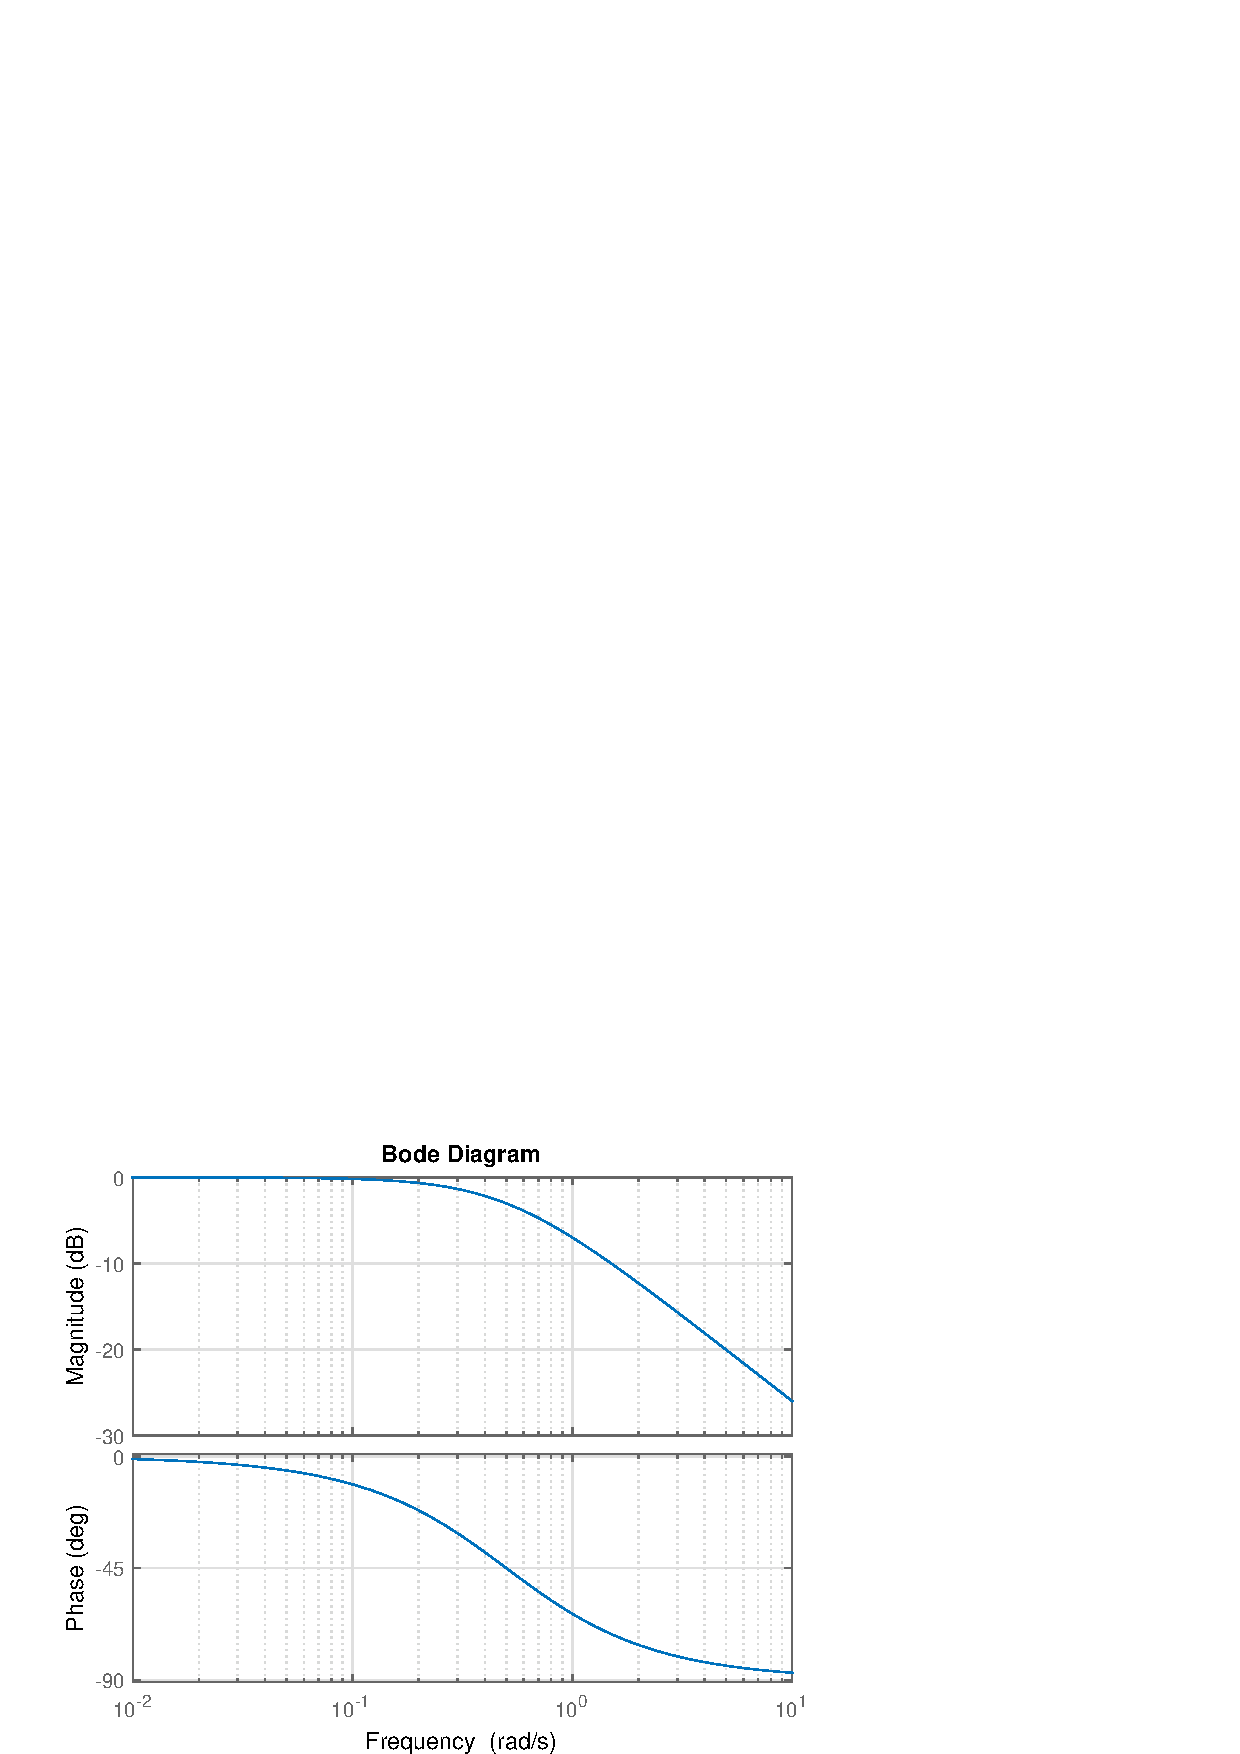
\includegraphics[width=\columnwidth]{smooth-bode}
\label{fig:smooth-bode}
\end{figure}
\end{minipage}
\begin{minipage}{0.2\linewidth}
	\[\frac{Y(s)}{R(s)} = \frac{0.5}{s+0.5}\]
\end{minipage}

\hspace*{-2em}
\begin{minipage}{0.7\linewidth}
\begin{figure}
\centering
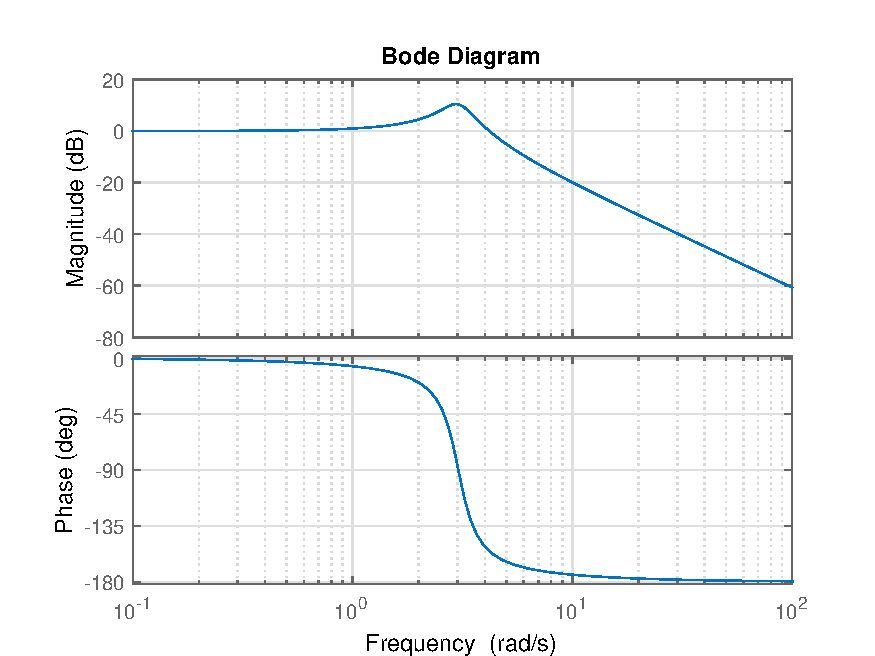
\includegraphics[width=\columnwidth]{osc-bode}
\label{fig:osc-bode}
\end{figure}
\end{minipage}
\begin{minipage}{0.2\linewidth}
	\[\frac{Y(s)}{R(s)} = \frac{10}{1.09s^2 + s + 10}\]
\end{minipage}
\end{frame}


\begin{frame}
	\frametitle{Exercise: Which controller do you prefer?}
	The output $Y(s)$ of the closed-loop system when $R(s)$ is a step function is as follows:
	\hspace*{-1em}
	\begin{minipage}{0.7\linewidth}
	\begin{figure}
		\centering
		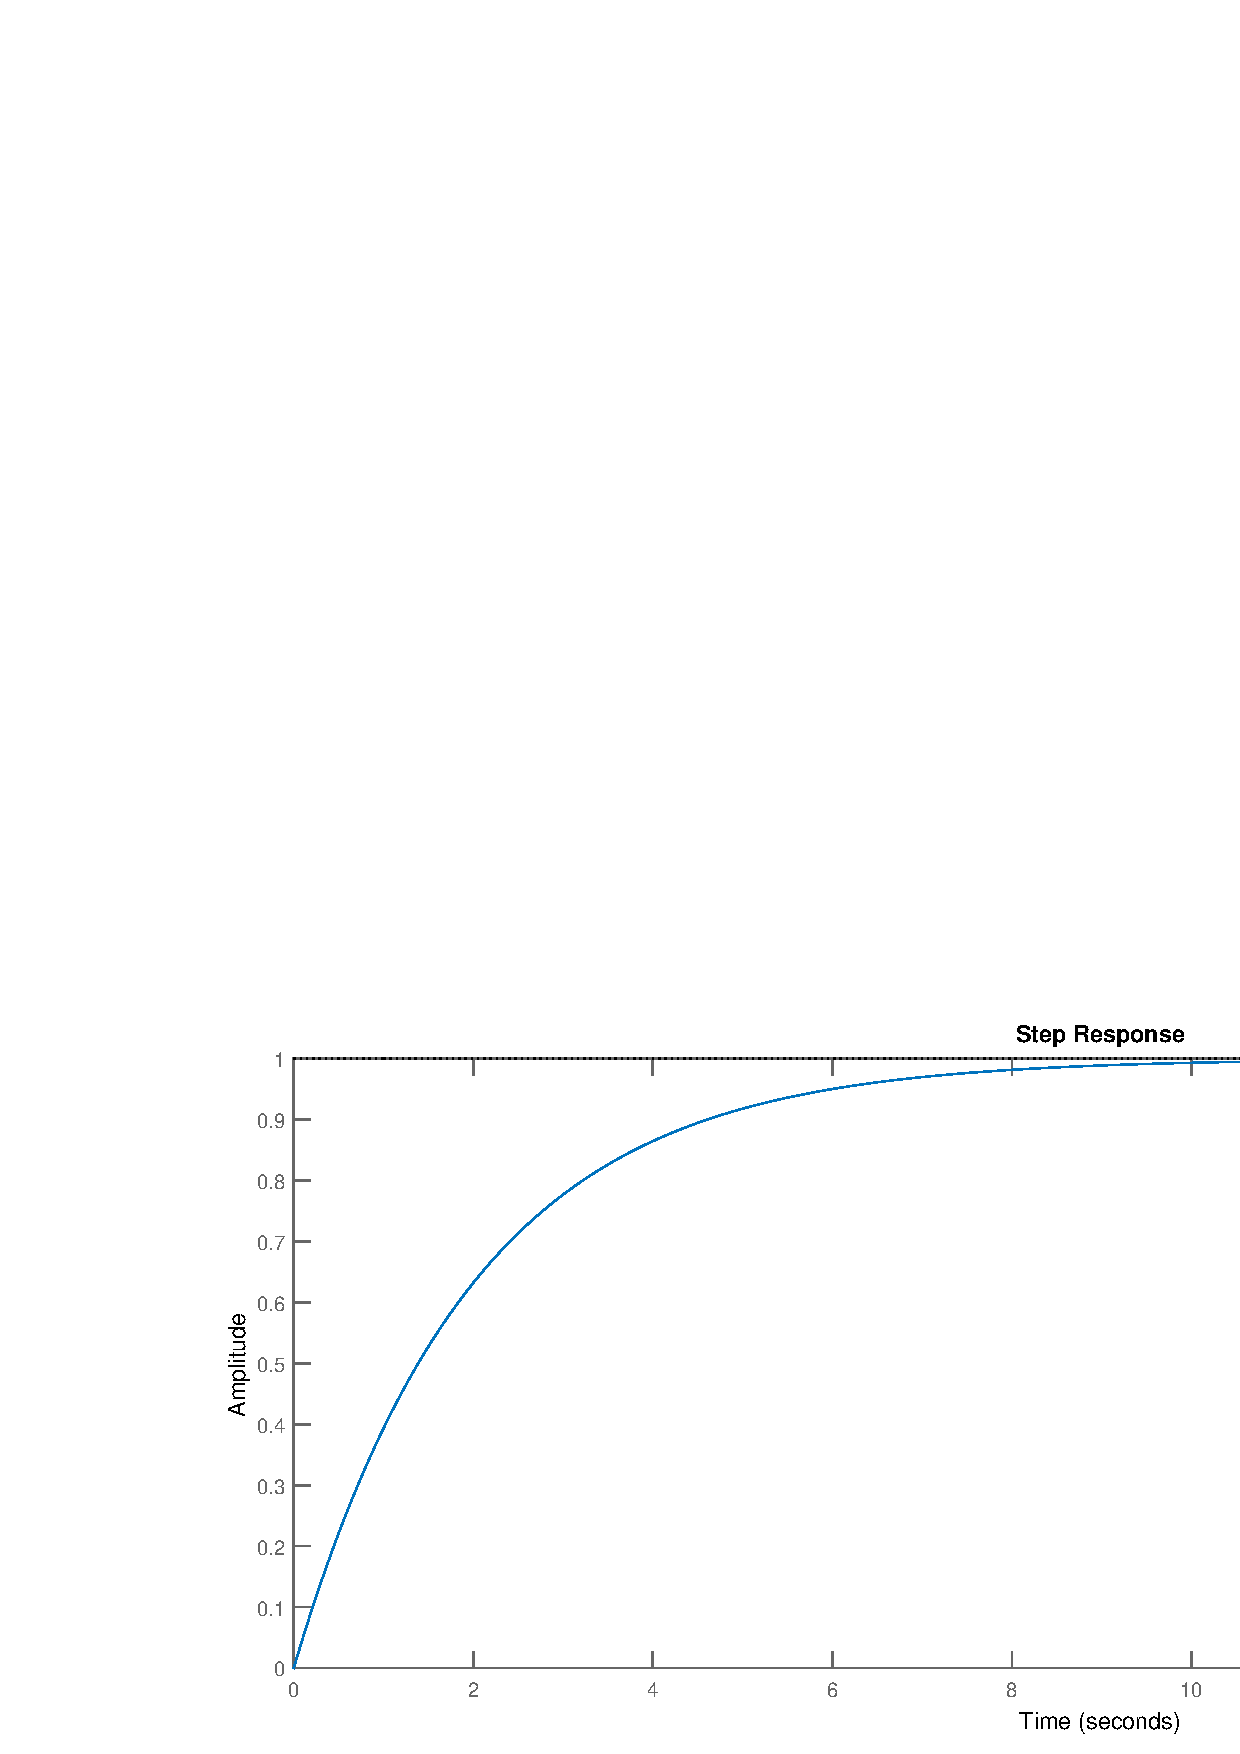
\includegraphics[width=\columnwidth]{smooth-step}
		\label{fig:smooth-step}
	\end{figure}
\end{minipage}
\begin{minipage}{0.2\linewidth}
		\[\frac{Y(s)}{R(s)} = \frac{0.5}{s+0.5}\]
\end{minipage}
\hspace*{-1em}
	\begin{minipage}{0.7\linewidth}
			\begin{figure}
				\centering
				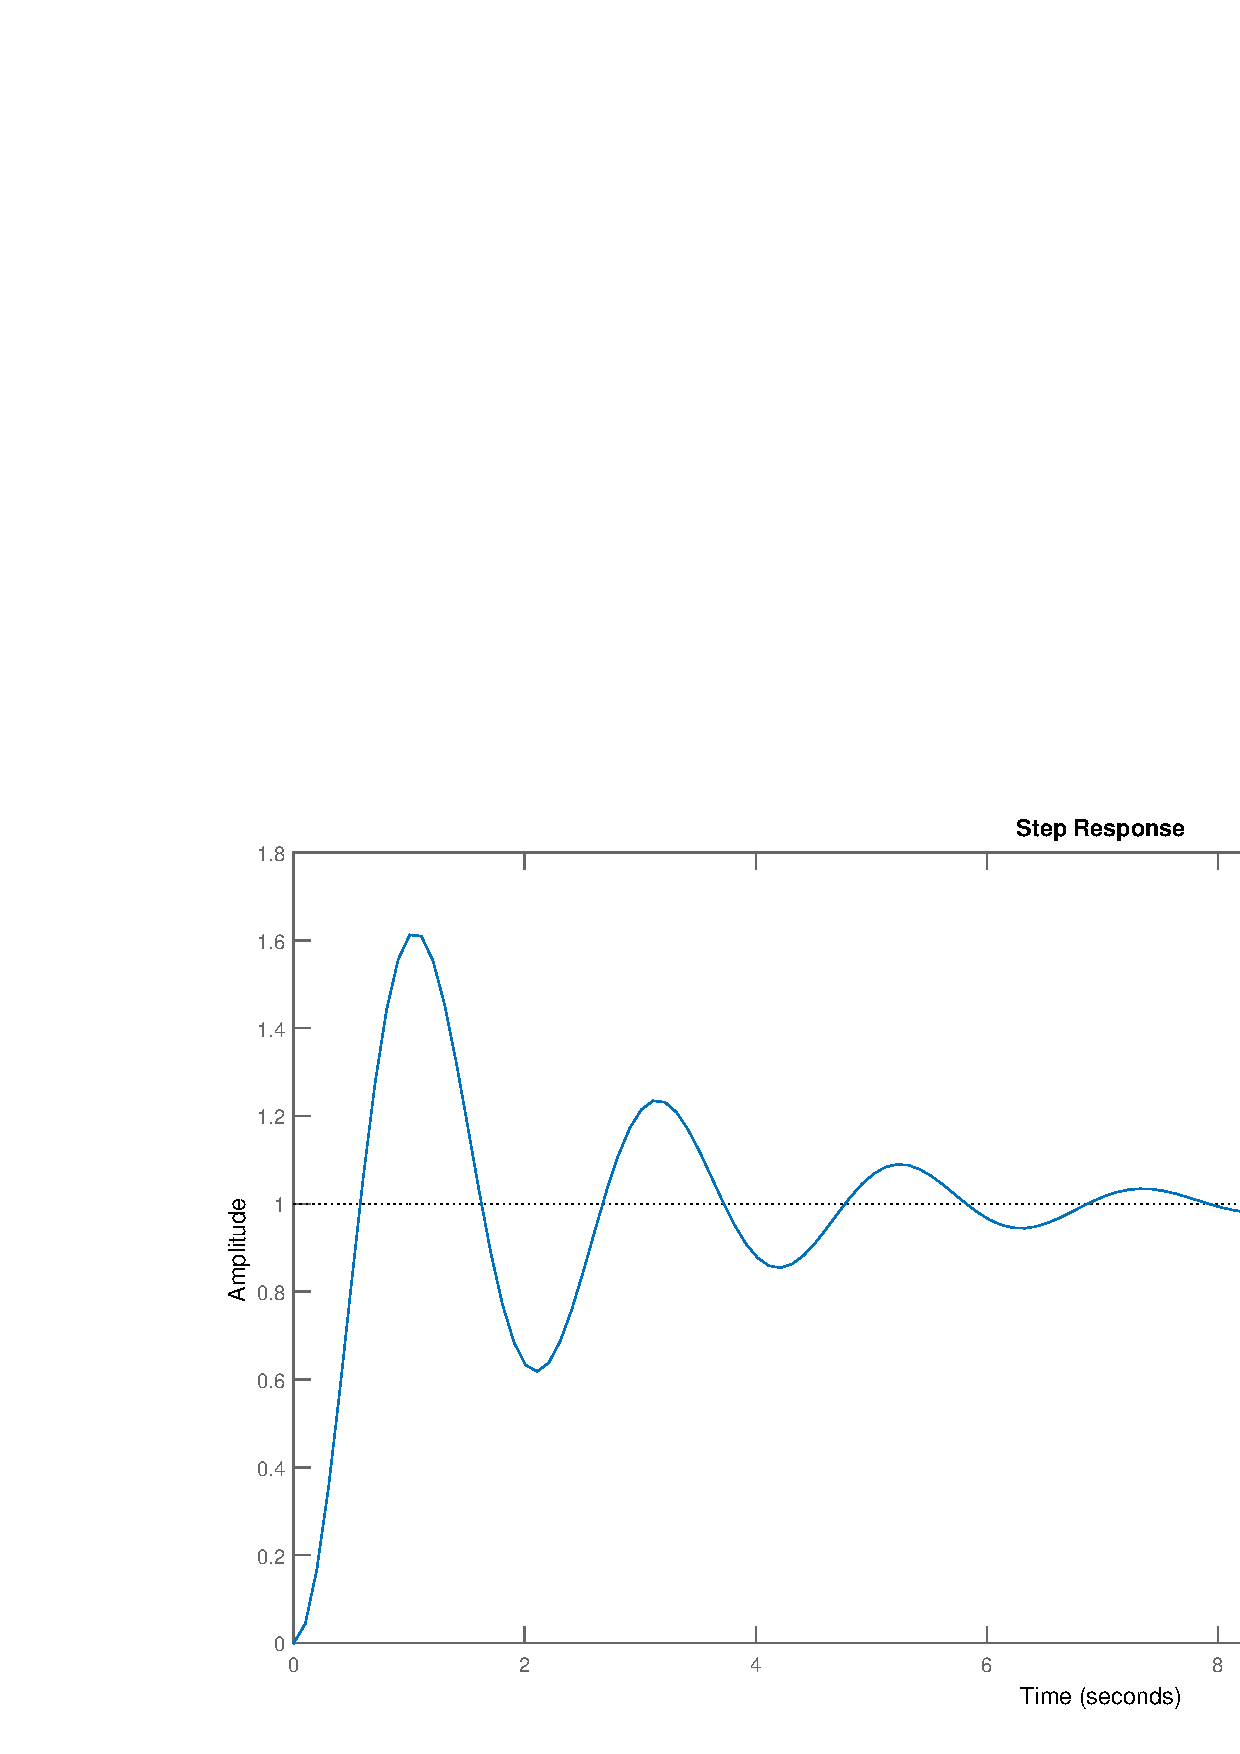
\includegraphics[width=\columnwidth]{osc-step}
				\label{fig:osc-step}
			\end{figure}
	\end{minipage}
	\begin{minipage}{0.2\linewidth}
			\[\frac{Y(s)}{R(s)} = \frac{10}{1.09s^2 + s + 10}\]
		\end{minipage}
\end{frame}

\begin{frame}
	\frametitle{Quality of reference tracking}
	\begin{minipage}{0.5\linewidth}
		\begin{block}{}
			Look at the step response of the transfer function from $R(s)$ to $Y(s)$. The quality can be determined using these criteria:
			\begin{itemize}
				\item Rise-time
				\item Settling time
				\item Steady-state error
				\item Overshoot
				\item ...
			\end{itemize}
		\end{block}
	\end{minipage}
	\hfill
	\begin{minipage}{0.4\linewidth}
		\begin{figure}
			\centering
			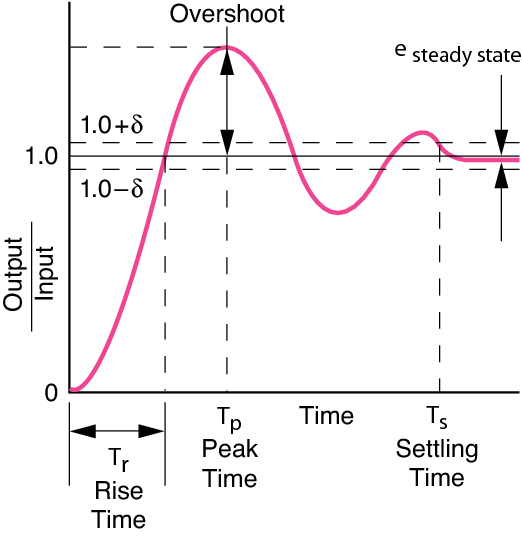
\includegraphics[width=1\linewidth]{properties}
			\label{fig:properties}
		\end{figure}
	\end{minipage}
\end{frame}

\begin{frame}
	\frametitle{Model errors}
	\begin{block}{}
		\begin{itemize}
			\item The plant characteristics may be variable or time-varying.
			System modeling techniques identify the plant
			within a certain model class and with a certain amount
			of inaccuracy. So there always exists a plant uncertainty,
			which cannot be described exactly by the mathematical
			models.	
			\item Control systems need to be made robust against this
			plant variability and uncertainty.
		\end{itemize}
	\end{block}
\end{frame}


\subsection[Sensitivity - Robustness]{Sensitivity - Robustness}
\begin{frame}
	\frametitle{Sensitivity}
	\begin{block}{}
		Sensitivity is a measure of the relative change in the system due to a relative change in a chosen parameter. Here we look at \small{$\Delta Y(s)$} due to \small{$\Delta P(s)$}.
		
		\begin{scriptsize}
		\begin{flalign*}
		Y(s) + \Delta Y(s) &= \frac{(P(s) + \Delta P(s))C(s)}{1+(P(s) + \Delta P(s))C(s)}R(s) + \frac{1}{1+(P(s) + \Delta P(s))C(s)}D(s)
		\end{flalign*}
		\end{scriptsize}
	\end{block}
	\begin{block}{}
		Look at the effect on the system without disturbances ($D(s)$=0)
		\begin{flalign*}
			\Delta Y(s) &= \frac{(P(s)+\Delta P(s))C(s)}{1 + (P(s) + \Delta P(s))C(s)}R(s) - \frac{P(s)C(s)}{1+P(s)C(s)}R(s) \\
		\end{flalign*}
	\end{block}
\end{frame}

\begin{frame}
	\frametitle{Sensitivity}
	\begin{block}{}
		\fontsize{7.5 pt}{9 pt}
		\begin{flalign*}
			&= \frac{(P(s)+\Delta P(s))C(s)(1+P(s)C(s)) - P(s)C(s) - P(s)C(s)(P(s) + \Delta P(s))C(s)}{(1+(P(s) + \Delta P(s))C(s)(1 + P(s)C(s))}R(s) \\
			&= \frac{\Delta P(s)C(s)}{(1+(P(s) + \Delta P(s))C(s))(1+P(s)C(s))}R(s) \\
			&= Y(s) \frac{\Delta P(s)}{P(s)} \frac{1}{1 + (P(s) + \Delta P(s))C(s)}
		\end{flalign*}
	\end{block}
\end{frame}


\begin{frame}
	\frametitle{Sensitivity}
	\begin{alertblock}{}
		Now take the relative change due to this model uncertainty and take the limit for $\Delta x \rightarrow 0$; this gives the following (measure of the) sensitivity:
		\begin{align*}
			S_P^Y(s) &= \frac{\frac{\partial Y}{Y}(s)}{\frac{\partial P}{P}(s)} = \frac{\partial Y}{\partial P}\left(s\right) \cdot \frac{P(s)}{Y(s)} = \frac{1}{1 + P(s)C(s)}
		\end{align*}
	\end{alertblock}
	\begin{block}{}
		\begin{itemize}
			\item Again, a very large $\left|P(s)C(s)\right|$ looks like a good choice, but again there is a risk for instability!
			\item Note that the sensitivity can be determined for any parameter	
		\end{itemize}
	\end{block}
\end{frame}

\begin{frame}
	\frametitle{Example 1}
	\begin{exampleblock}{Problem statement}
		Suppose we want to stabilize the system $P(s)=\frac{1}{(s - a)}$.  We only know that $a \in [0.20;0.80]$. We propose to use a proportional controller $C(s)=K$.
		The closed-loop transfer function becomes
		\begin{align*}
			H(s) = \frac{P(s)C(s)}{1+P(s)C(s)} = \frac{\frac{1}{s-a}K}{1+\frac{1}{s-a}K} = \frac{K}{s-a+K}
		\end{align*}
		The controller stabilizes the system if $ - a+K>0$. If we choose $K$ very large the system will be robust against changes in $a$.
		
	\end{exampleblock}
\end{frame}


\begin{frame}
	\frametitle{Example 2}
	\begin{example}
		Suppose we want to stabilize the system $P(s)=\frac{s}{(s - a)}$ with $a\in[0.20;0.80]$. If we choose the control law $C(s)=\frac{K}{s}$ this results in the same transfer function.
		\vspace{-0.5em}
		\begin{align*}
			H(s) = \frac{P(s)C(s)}{1+P(s)C(s)} = \frac{\frac{s}{s-a}\frac{K}{s}}{1+\frac{s}{s-a} \frac{K}{s}} = \frac{K}{s-a+K}
		\end{align*}
		Again we choose $K>a$ to ensure stability.
		But how does the controller perform on the slightly perturbed system $\tilde{P}(s)=\frac{(s+\epsilon)}{(s - a)}$  ?
		The transfer function from $R(s)$ to $Y(s)$ becomes
				\vspace{-0.5em}
		\begin{align*}
			\tilde{H}(s) = \frac{\frac{s+\epsilon}{s-a} \frac{K}{S}}{1+\frac{s+\epsilon}{s-a}\frac{K}{s}}
			= \frac{(s+\epsilon)K}{s^2 + (K-a)s + \epsilon K}
		\end{align*}
	\end{example}
\end{frame}

\begin{frame}
	\frametitle{Example 2}
	\begin{minipage}{0.5\linewidth}
		\begin{block}{}
			\vspace*{-1em}
			\begin{flalign*}
				\tilde{S}(s) = \frac{(s+\epsilon)K}{s^2 + (K-a)s + \epsilon K}
			\end{flalign*}
			The figure on the right plots
			\begin{flalign*}
				&{\color{blue} s^2 + (K - a)s} \\
				&{\color{red} s^2 + (K - a)s + \epsilon K}
			\end{flalign*}
			For $\epsilon$ negative the system becomes unstable. The control system is not robust and useless in practical situations. You should not use control laws which rely on a pole-zero cancellation. 
		\end{block}
	\end{minipage}
	\hspace{0.1em}
	\begin{minipage}{0.4\linewidth}
		\begin{figure}
			\center
			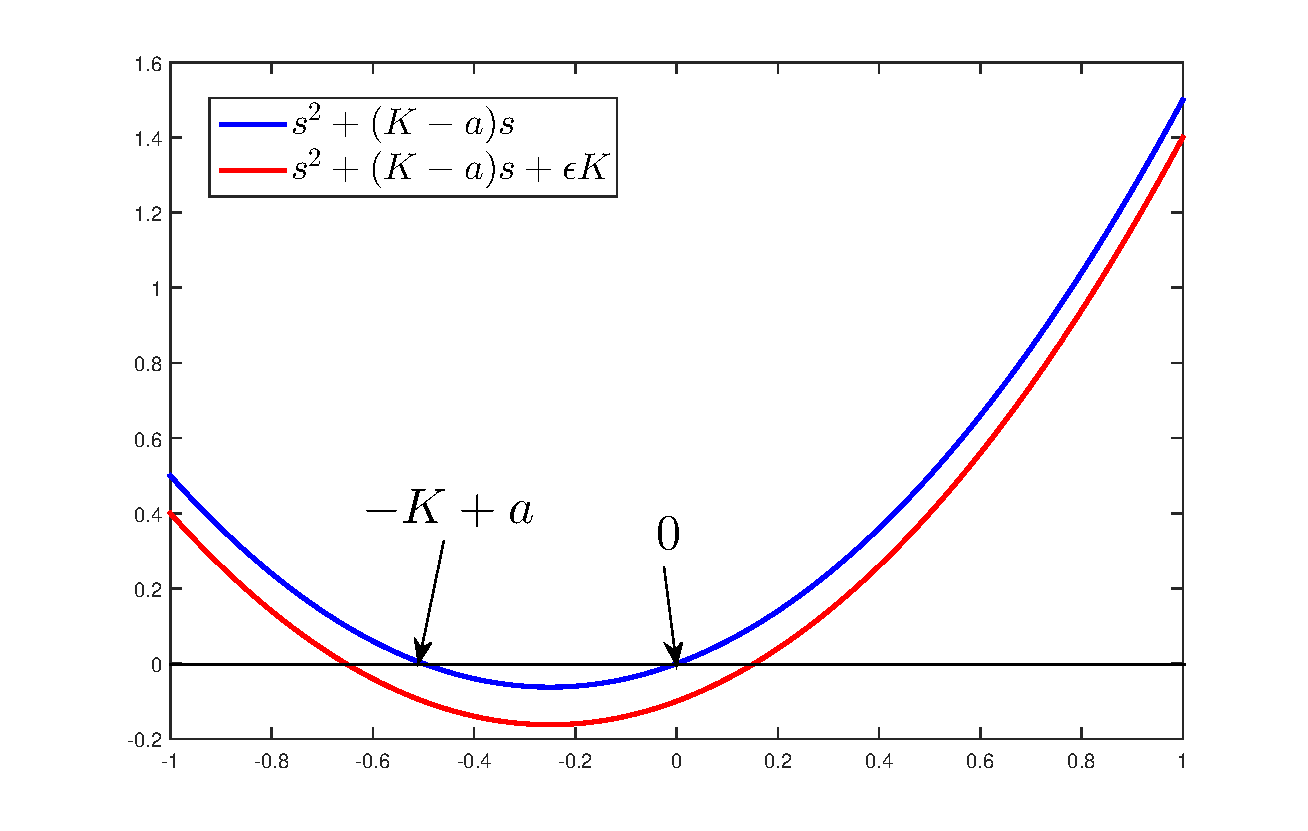
\includegraphics[width=1.5\linewidth]{robustnessexample}
			\label{fig:robustness-example}
		\end{figure}
	\end{minipage}
\end{frame}


\begin{frame}
	\frametitle{Sensitivity - Robustness}
	\begin{block}{Steady-state error}
		The steady state error is defined as follows:
		\begin{align*}
			\lim\limits_{t \rightarrow \infty} e(t)
			&= \lim\limits_{t \rightarrow \infty} (r(t) - y(t)) \\
			&= \lim\limits_{s \rightarrow 0} s(R(s) - Y(s)) &\text{(final value theorem)}
		\end{align*}
		A very small steady state error (preferably zero) indicates that the controller tracks the reference very well.
	\end{block}
\end{frame}


\begin{frame}
	\frametitle{Sensitivity - Robustness}
	\begin{block}{Open-loop system}	
		For an open loop system with a step reference, the steady-state error is given by
		\begin{align*}
			e_{ol}(\infty) &= \lim\limits_{s \rightarrow 0}
			s(1 - C(s)P(s))R(s) = 1 - C(0)P(0)
		\end{align*}
		\vspace{-1em}
		\begin{itemize}
			\item So, the open loop system has no steady state error (for a step reference) if the controller is calibrated such that $C(0)P(0)=1$
			\item $\Rightarrow$ a precise calibration of the DC gain (not robust)
		\end{itemize}
	\end{block}
\end{frame}


\begin{frame}
	\frametitle{Sensitivity - Robustness}
	\begin{block}{Closed-loop system}
		The steady-state error for a step reference is given by
		\begin{flalign*}
			e_{cl}(\infty) &= \lim\limits_{s \rightarrow 0} s\left(1 - \frac{C(s)P(s)}{1+C(s)P(s)}\right)R(s) \\
			&= \lim\limits_{s \rightarrow 0} \frac{s}{1 + C(s)P(s)}R(s) = \frac{1}{1+C(0)P(0)}
		\end{flalign*}
		\begin{itemize}
			\item The steady state error is small if $C(0)P(0)$ is very large
			\item Again, calibrating the DC gain
			\item The difference is that we only need a large gain, which is far less demanding than having to make it equal to 1
		\end{itemize}
	\end{block}
\end{frame}

\begin{frame}
	\frametitle{An open loop controller is not robust}
	\begin{block}{}
		We can now show how this results in a great advantage of the closed-loop strategy over the open loop strategy:
		\begin{itemize}
			\item If $P$ changes slightly (for instance due to a factor that has not been taken up into the model) to $P+\Delta P$
			\item Then making $e_{ol}(\infty)$ small would require to calibrate anew
			\item Whereas $e_{cl} (\infty)$ would remain small, as long as $(P(0)+\Delta P(0))C(0)$ remains large
			
		\end{itemize}
		Hence an open loop configuration can not control the output \textbf{robustly} against changes in $P$
	\end{block}
\end{frame}

\subsection[Types of systems and SS-error]{Types of systems and Steady State Error}

\begin{frame}
	\frametitle{Steady state error: step}
	\begin{definition}
		\begin{minipage}{0.4\linewidth}
			\[
			\epsilon (t) =
			\begin{cases}
			0, \quad t \leqslant 0 \\
			\frac{1}{2}, \quad t = 0 \\
			1, \quad t \geqslant 0
			\end{cases}
			\]
		\end{minipage}
		\begin{minipage}{0.5\linewidth}
			\hspace*{4em}
			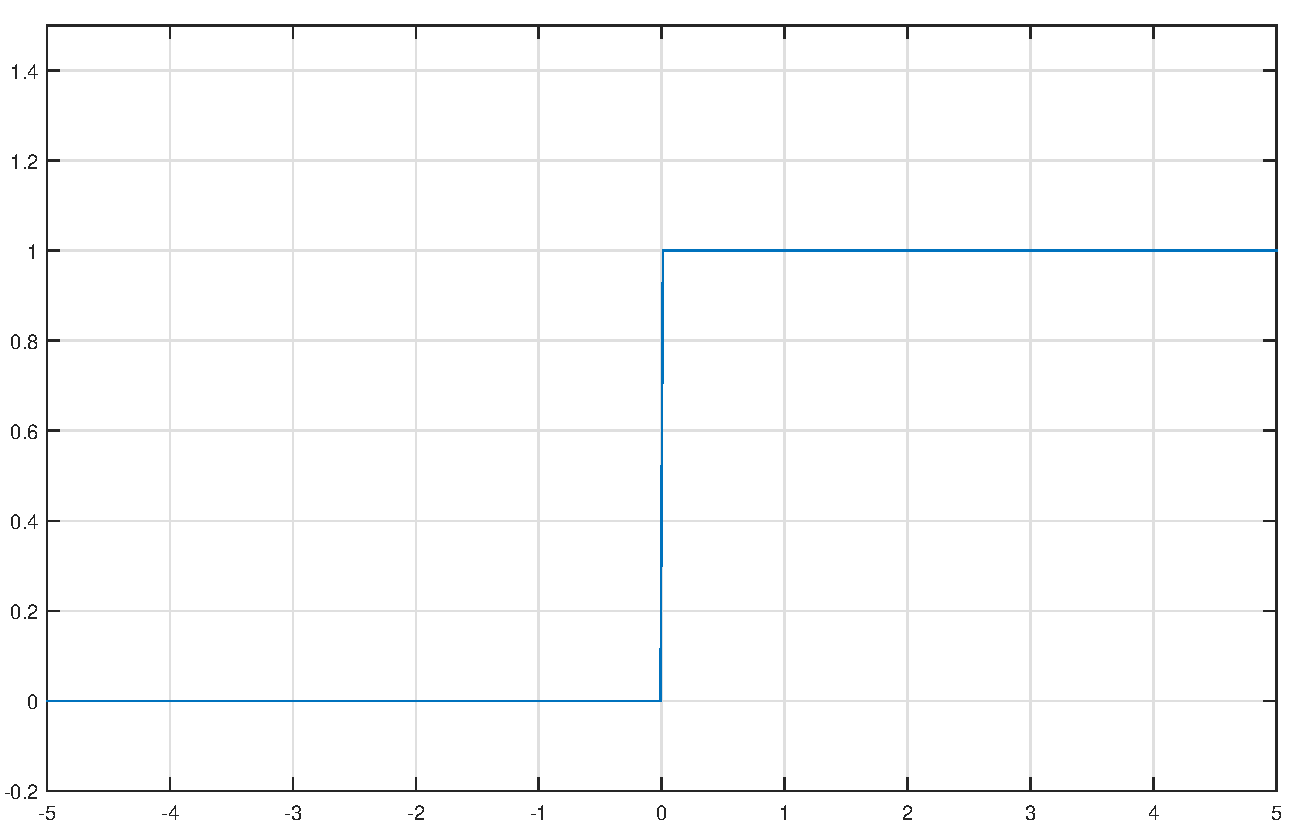
\includegraphics[width=0.6\linewidth]{stepfunc}
		\end{minipage}
	\end{definition}
	\begin{block}{}
		For a step reference $r(t) = a \epsilon (t)$ $\Rightarrow R(s) = \frac{a}{s}$
		\[e_{cl}(\infty) = \frac{s}{1+C(0)P(0)} \frac{a}{s}\]
		So $e_{cl}(\infty) = 0$ if C(s)P(s) has a least one pole in zero ($C(0)P(0) \rightarrow \infty$)
	\end{block}
\end{frame}

\begin{frame}
	\frametitle{Steady state error: ramp}
	\begin{block}{}
		For a ramp reference function $r(t) = at \epsilon (t) \, \Rightarrow R(s) = \frac{a}{s^2}$, we have
		\begin{flalign*}
			e_{cl}(\infty) = \lim\limits_{s \rightarrow 0} \frac{s}{1+C(s)P(s)} \frac{a}{s^2}
		\end{flalign*}
		So, $e_{cl}(\infty) = 0$ if $C(s)P(s)$ has at least two poles in zero. $\left(\lim\limits_{s\rightarrow 0} sC(s)P(s) = \infty\right)$
	\end{block}
\end{frame}

\begin{frame}
	\frametitle{Type of a system}
	\begin{block}{}
		\begin{itemize}
			\item The type of a system is determined by the number of poles $P(s)C(s)$ has in zero, and hence it is linked to what type of references it can track perfectly
			\item Write $P(s)C(s)$ as $\frac{K \prod_{k=1}^{m} (s-z_k)}{s^i \prod_{k=1}^{n-i} (s-p_k)}$ with $i$ the amount of poles in zero
			\item We say this system is of type $i$
			\begin{itemize}
				\item It will be able to track references of shape $at^0 \epsilon(t)$ up to $at^{i - 1} \epsilon(t)$ perfectly for $t\rightarrow \infty$ ($\lim\limits_{t \rightarrow \infty} e_{cl}(t) = 0$)
				\item A reference of shape $at^i \epsilon(t)$ will be missed by a finite factor for $t\rightarrow \infty$ ($\lim\limits_{t \rightarrow \infty} e_{cl}(t) = C$)
				\item A reference of shape $at^{i+1} \epsilon(t)$, $at^{i+2} \epsilon(t)$, ... will be missed by infinity for $t\rightarrow \infty$ ($\lim\limits_{t \rightarrow \infty} e_{cl}(t) = \infty$)
			\end{itemize}
		\end{itemize}
	\end{block}
\end{frame}

\begin{frame}
	\frametitle{Example of a type 0 system}
		\begin{example}
			{Step reference $r(t) = a \epsilon (t) \Rightarrow R(s) = \frac{a}{s}$}
			\begin{flalign*}
				e_{cl}(\infty) &= \lim\limits_{s \rightarrow 0} \frac{s}{1 + C(s)P(s)} \frac{a}{s} \\
				&= \lim\limits_{s \rightarrow 0} \frac{a}{1 +  \color{red}{\frac{K \prod_{k=1}^{m} (-z_k)}{\prod_{k=1}^{n-i} (-p_k)}}}
				= \frac{a}{1 + \color{red}{K_p}}
			\end{flalign*}
			where $K_p$ is the static position error constant
		\end{example}
\end{frame}

\begin{frame}
	\frametitle{Example of a type 0 system}
		\begin{example}
			{Ramp reference $r(t) = at \epsilon (t) \Rightarrow R(s) = \frac{a}{s^2}$}
			\begin{flalign*}
				e_{cl}(\infty) &= \lim\limits_{s \rightarrow 0} \frac{s}{1+C(s)P(s)} \frac{a}{s^2} \\
				&= \lim\limits_{s \rightarrow 0} \frac{1}{1 + \frac{K \prod_{k=1}^{m} (-z_k)}{\prod_{k=1}^{n-i} (-p_k)}} \frac{a}{s} \\
				&= \lim\limits_{s \rightarrow 0} \frac{a}{s + \color{red}{s \frac{K \prod_{k=1}^{m} (-z_k)}{\prod_{k=1}^{n-i} (-p_k)}}} = \frac{a}{\color{red}{K_v}} = \infty
			\end{flalign*}
			where $K_v$ is the static velocity error constant
		\end{example}
\end{frame}	

\begin{frame}
	\frametitle{Steady state errors - type of a system}
	\begin{block}{}
			\begin{tabbing}
			$K_p = \lim\limits_{s \rightarrow 0} P(s)C(s)$ 
			\hspace{2em} \= $K_p = $ Static position error constant \\
			$K_v = \lim\limits_{s \rightarrow 0}s P(s)C(s)$ \> $K_v = $ Static velocity error constant \\
			$K_a = \lim\limits_{s \rightarrow 0}s^2 P(s)C(s)$ \> $K_a = $ Static acceleration error constant
			\end{tabbing}
		\end{block}
	\begin{alertblock}{}
		And the respective steady state errors for different system types are: \\
		\vspace{1em}
		\centering
		\begin{tabular}{|l|c|c|c|}
			\hline \textbf{Type} $\mathbf{l}$ & \textbf{Step} $\mathbf{a \boldsymbol{\epsilon} (t)}$ & \textbf{Ramp} $\mathbf{at \boldsymbol{\epsilon} (t)}$ & \textbf{Parabola} $\mathbf{\frac{at^2 \boldsymbol{\epsilon} (t)}{2}}$ \\ 
			\hline \textbf{0} & $\frac{A}{1 + K_p}$ & $\infty$ & $\infty$ \\ 
			\hline \textbf{1} & 0 & $\frac{A}{K_v}$ & $\infty$ \\ 
			\hline \textbf{2} & 0 & 0 & $\frac{A}{K_a}$ \\ 
			\hline 
		\end{tabular} 
	\end{alertblock}
\end{frame}


\subsection[Noise and disturbance rejection]{Noise and disturbance rejection}

\begin{frame}
	\frametitle{Noise and disturbance rejection}
	\begin{block}{}
		\begin{itemize}
			\item Measurement noise is often modelled by zero-mean white noise.
			\item Disturbances are actual changes to the state of the system
		\end{itemize}
		\vspace{-1em}
		\begin{figure}
		\centering
		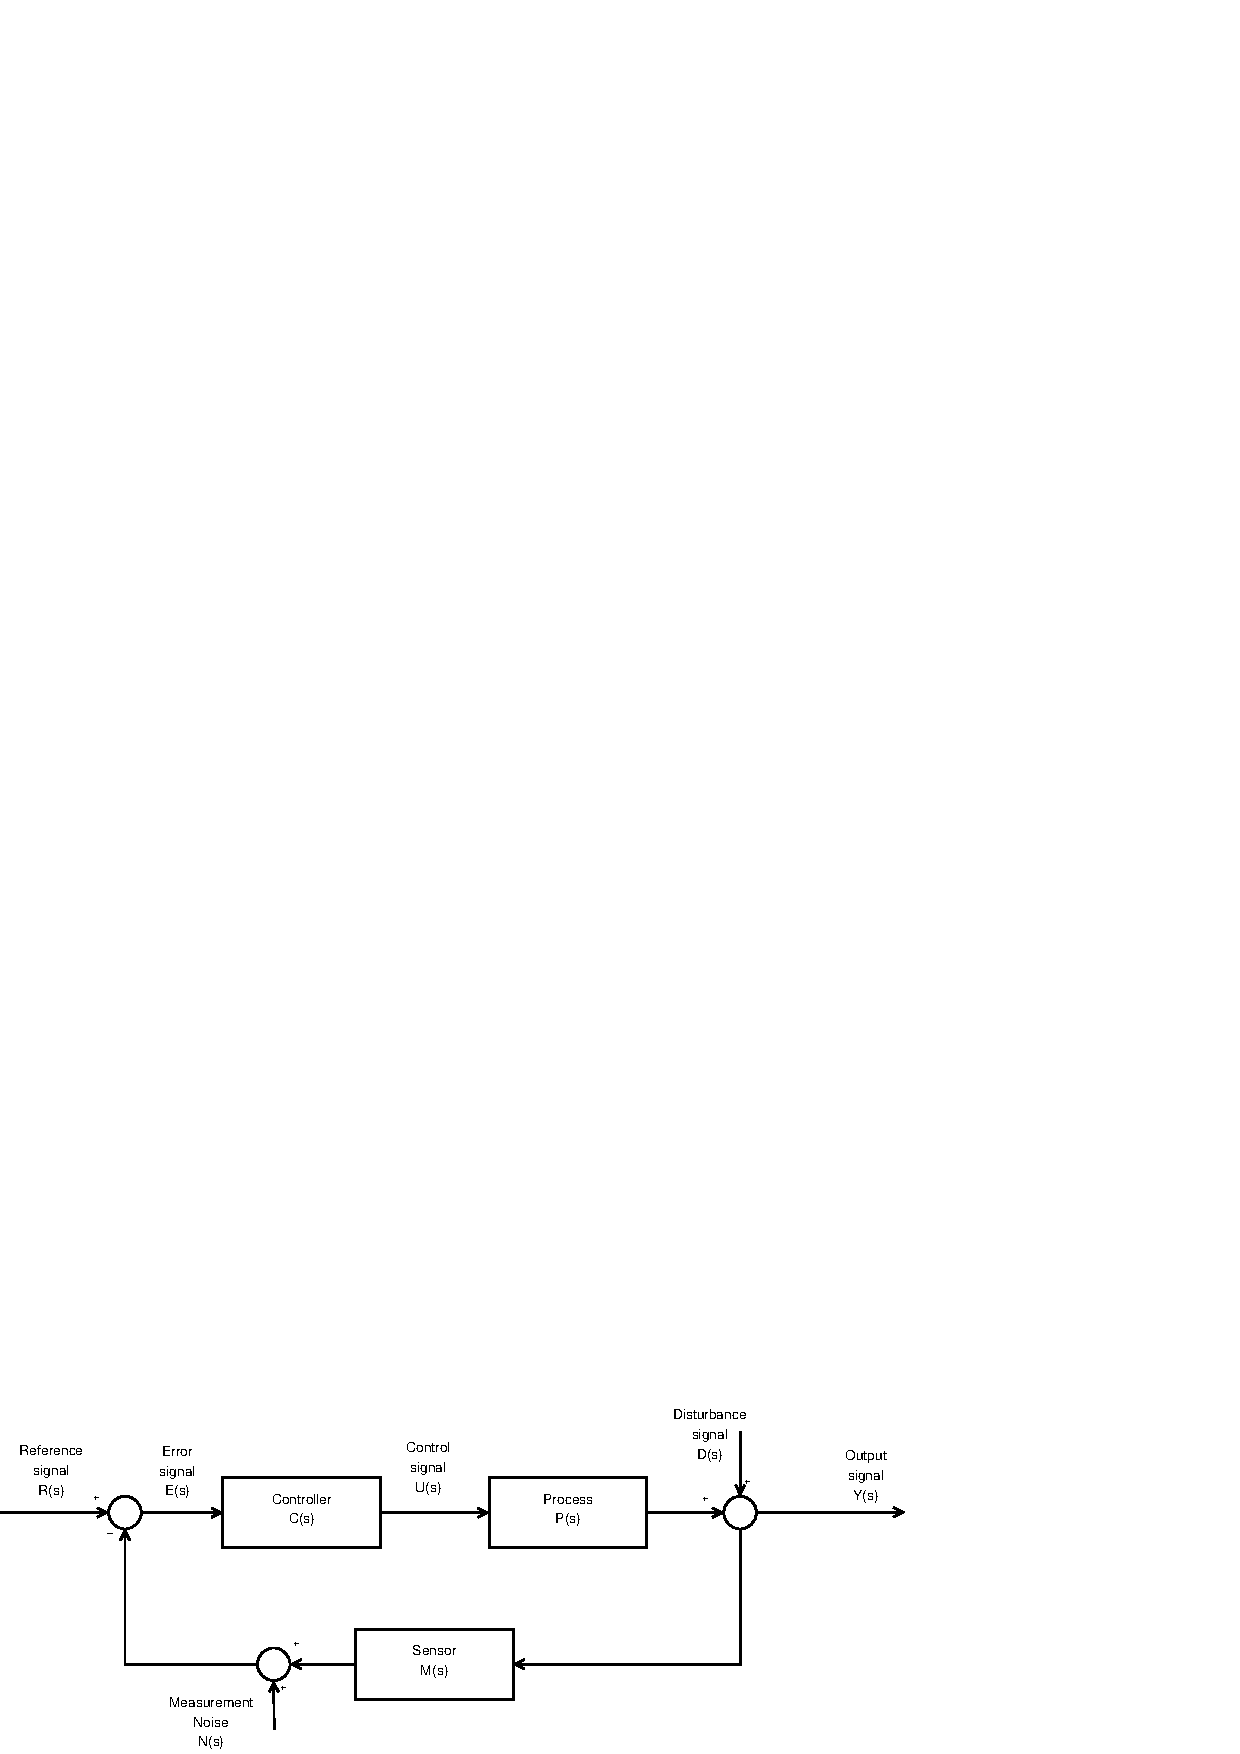
\includegraphics[width=0.8\linewidth]{Closed-Loop-measure}
		\label{fig:Closed-Loop3}
		\end{figure}
	\end{block}
\end{frame}


\begin{frame}
	\frametitle{Noise and disturbance rejection}
		\begin{itemize}
			\item Cruise control: \\
			\begin{itemize}
				\item Measurement errors on the speed are noise 
				\item A change in slope is a disturbance
			\end{itemize}
		\end{itemize}
		\begin{figure}
			\centering
			
\includegraphics[width=0.45\linewidth]{control-goals/steep-road}
			\label{fig:cruisecontrol}
		\end{figure}
\end{frame}

\begin{frame}
	\frametitle{Noise and disturbance rejection}
	\begin{block}{}
		\begin{itemize}
			\item Remember
			\vspace{-1em}
			\begin{figure}
				\centering
				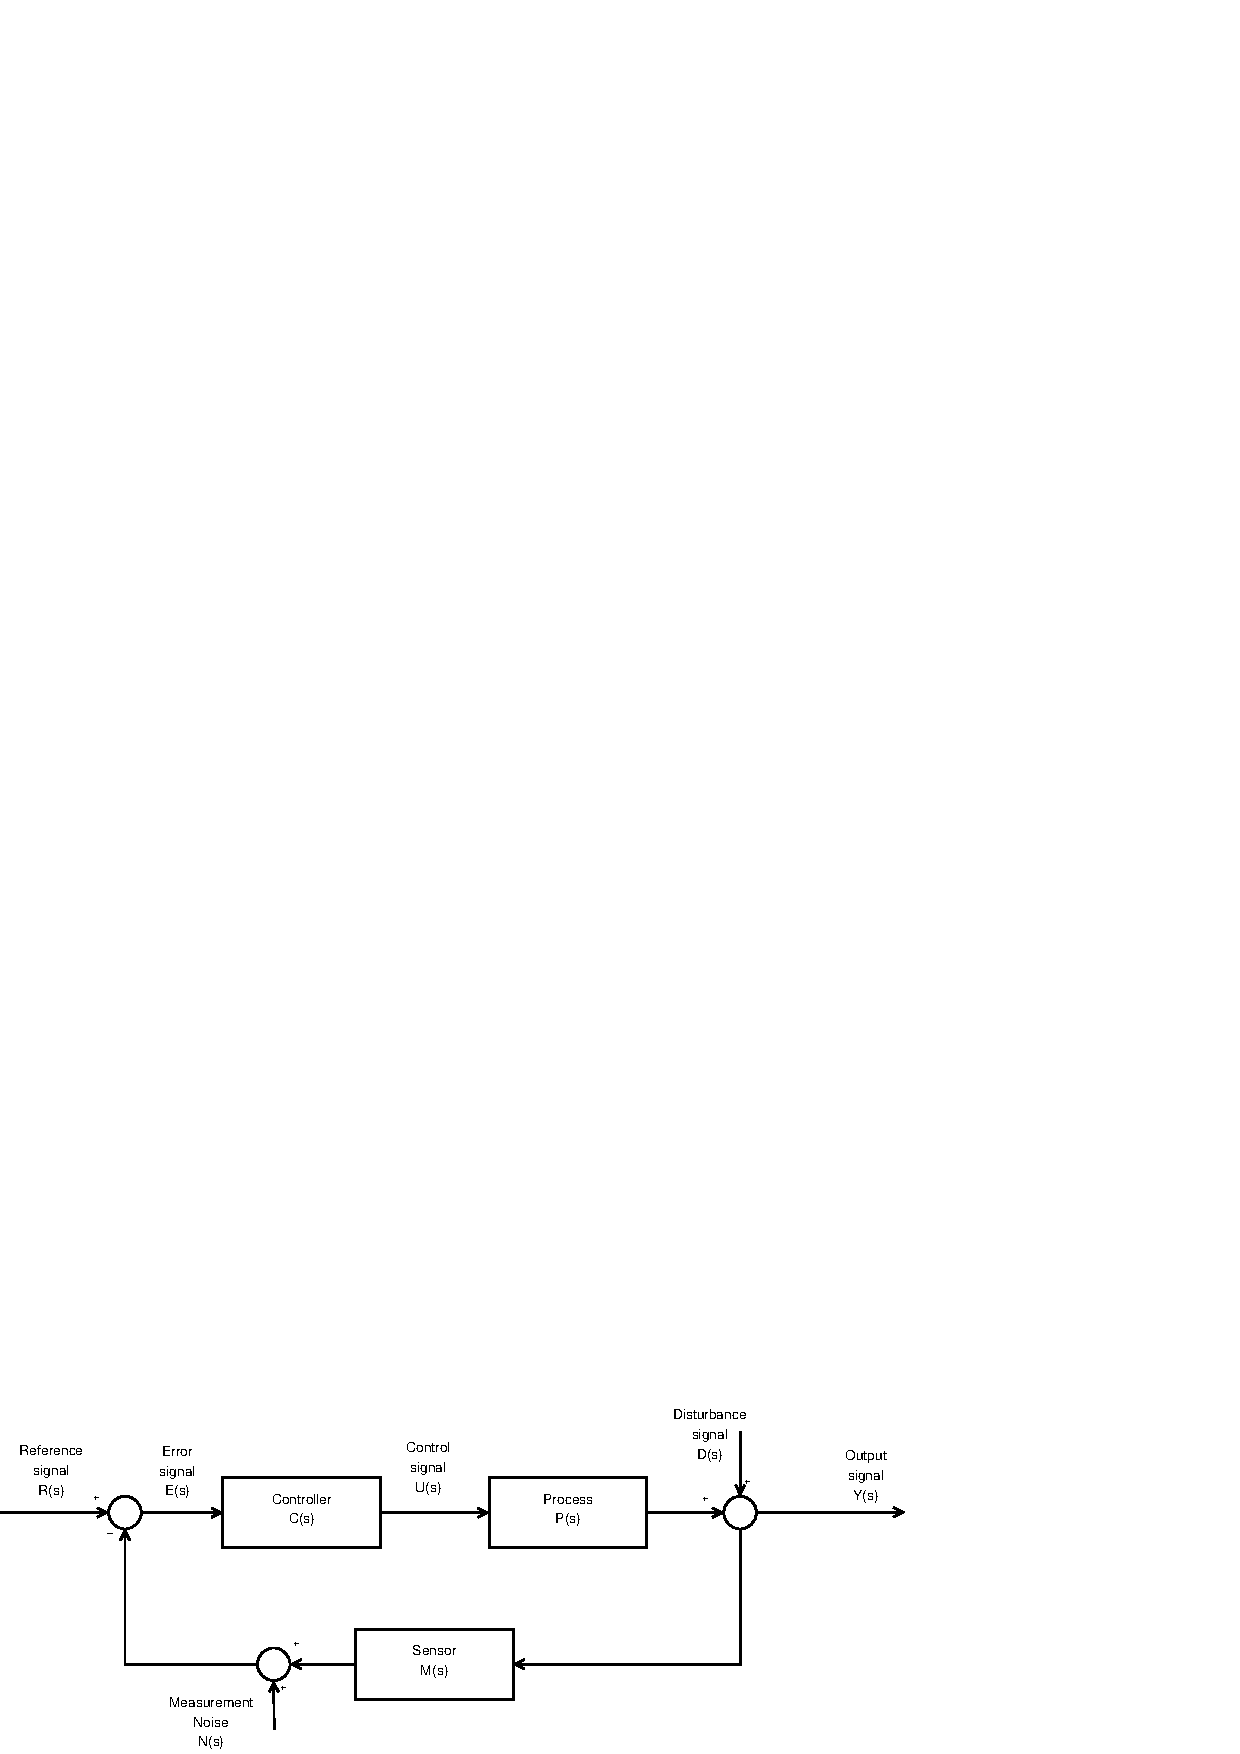
\includegraphics[width=0.9\linewidth]{Closed-Loop-measure}
				\label{fig:Closed-Loop4}
			\end{figure}
			\vspace{-1.5em}
			\begin{align*}
				Y(s) = \frac{P(s)C(s)}{1+P(s)C(s)}R(s) + \frac{1}{1+P(s)C(s)}D(s)
			\end{align*}
			\item Setting $M(s)=\frac{1}{1+P(s)C(s)}$ sufficiently small results in the rejection of $D$. This can be achieved by choosing $C(s)$ sufficiently high.
		\end{itemize}	
	\end{block}
\end{frame}


\begin{frame}
	\frametitle{Noise and disturbance rejection}
	\begin{block}{}
		\begin{itemize}
			\item What happens to the measurement noise?
			\begin{itemize}
				\item It will be amplified and applied to the input of the plant which in turn leads to a nervous controller.
			\end{itemize}
		\end{itemize}
		\begin{figure}
			\centering
			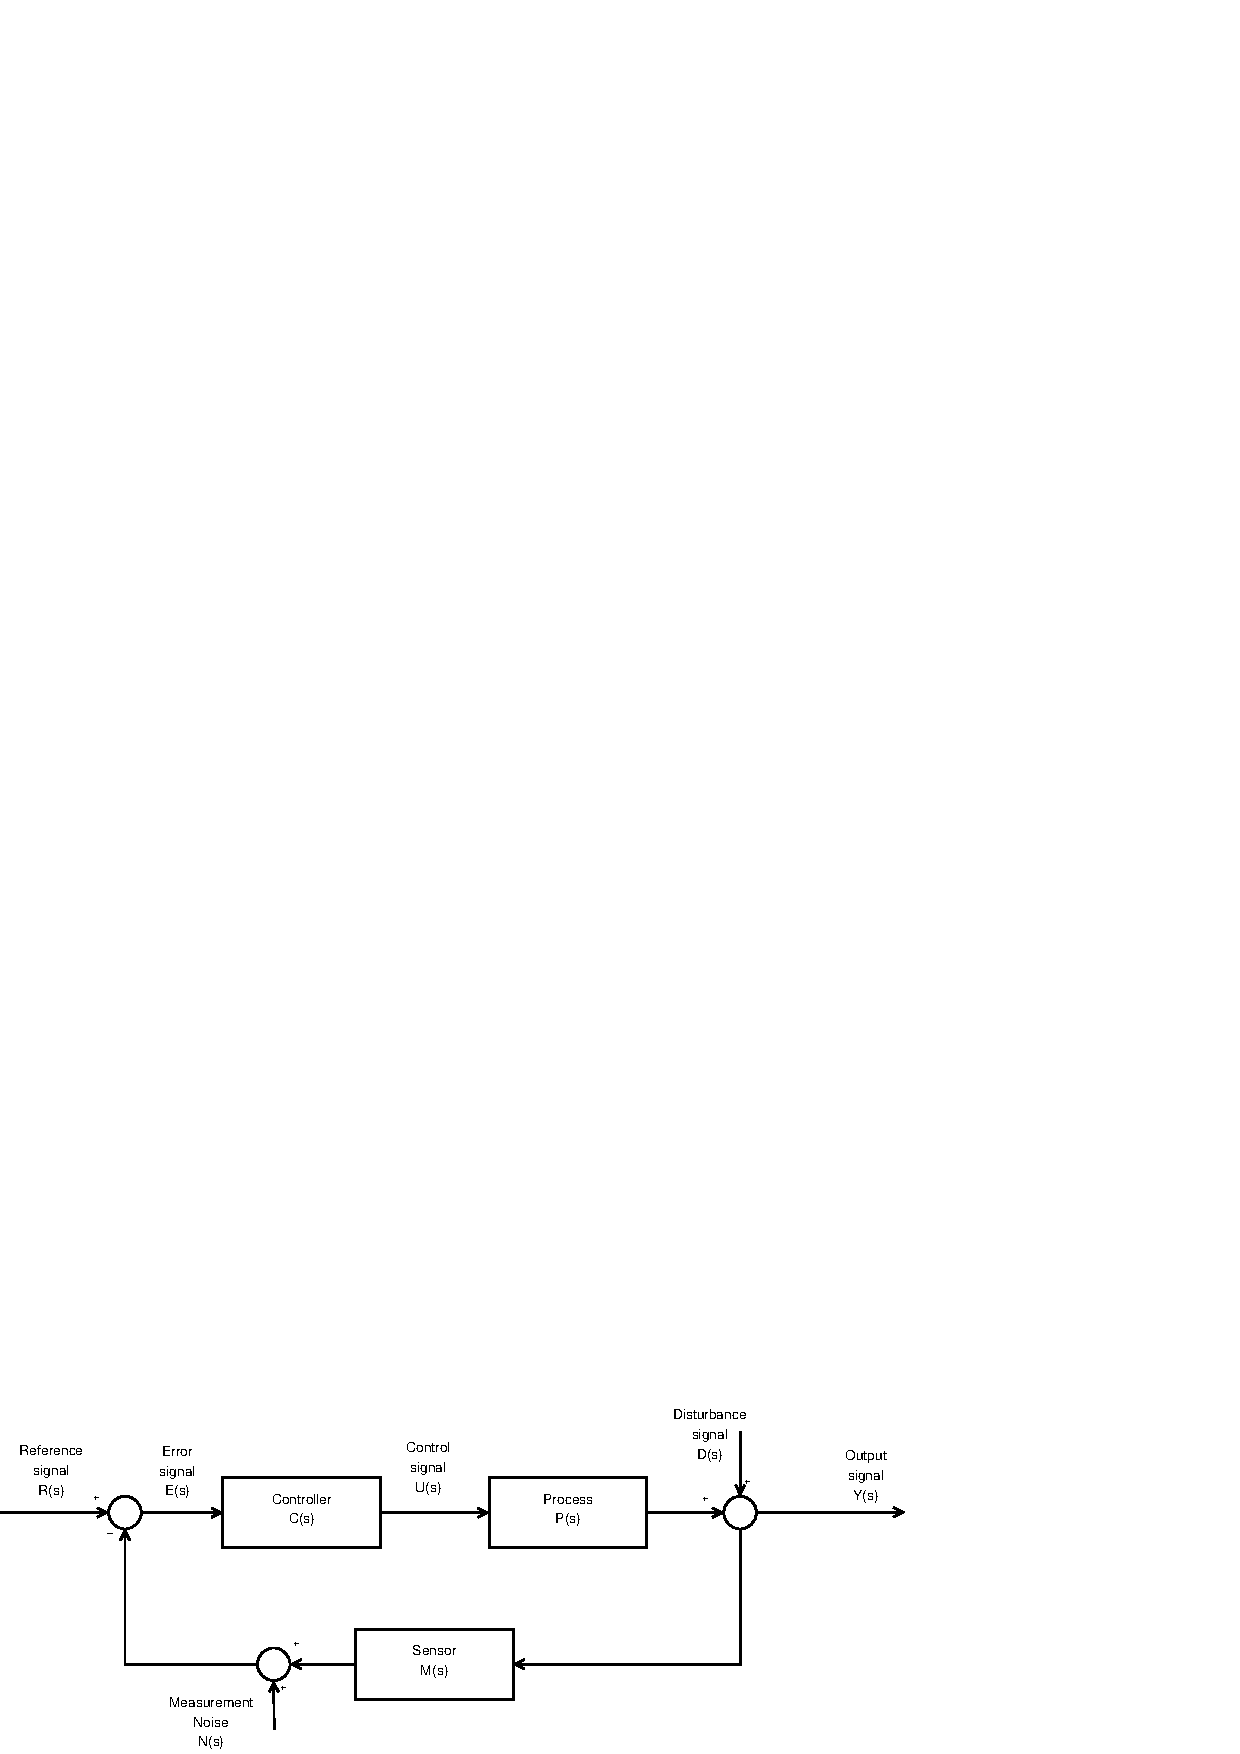
\includegraphics[width=0.8\linewidth]{Closed-Loop-measure}
			\label{fig:Closed-Loop5}
		\end{figure}
	\end{block}
\end{frame}


\begin{frame}
	\frametitle{Noise and disturbance rejection}
	\begin{block}{}
		\begin{itemize}
			\item Good disturbance rejection requires fast control actions to bring the system back to the desired state
			\item Good noise rejection requires slow control actions
			\item Note that a controller can not see the difference between measurement noise and disturbances. Slow controllers will be less sensitive to measurement noise but fast controllers will have better disturbance rejection
		\end{itemize}
	\end{block}
\end{frame}

\begin{frame}
	\begin{figure}
		\centering
		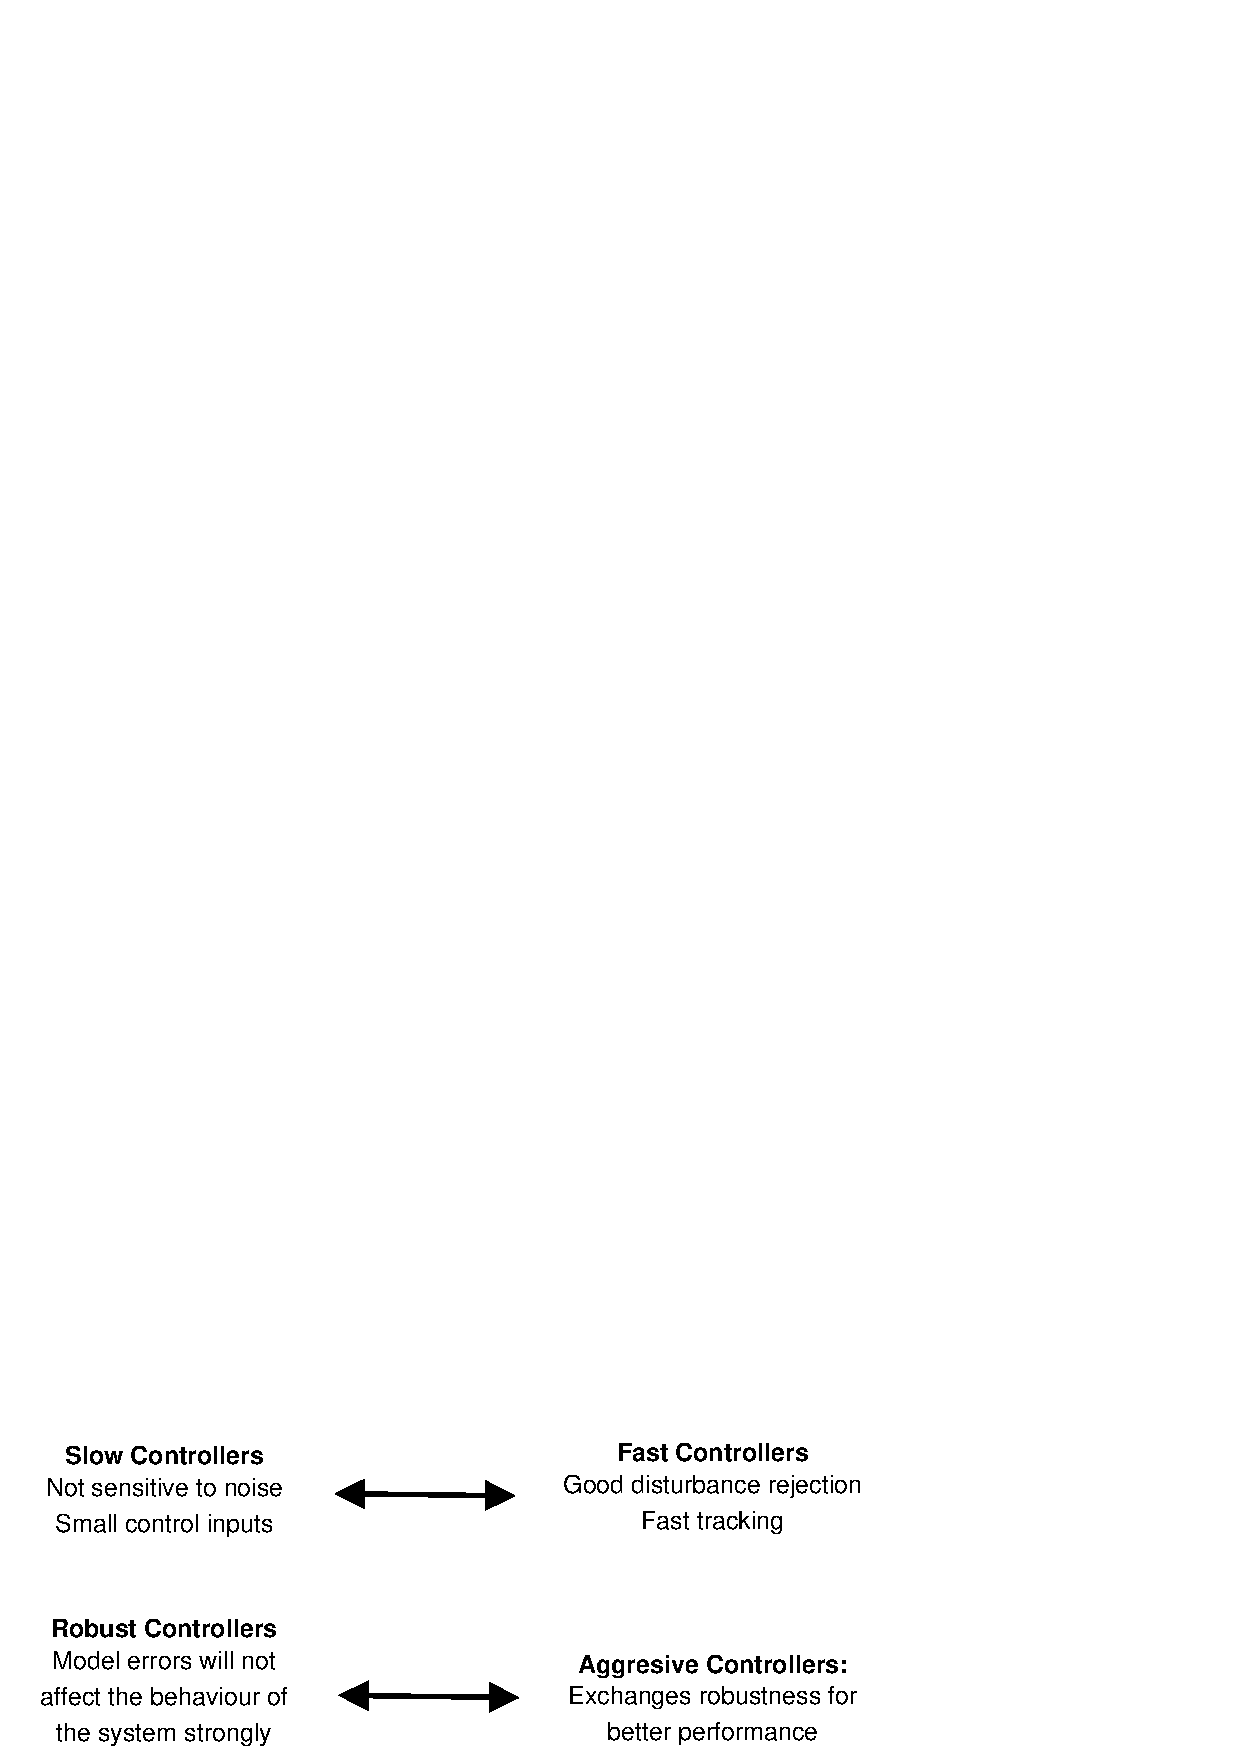
\includegraphics[width=1.1\linewidth]{comparison}
		\caption{}
		\label{fig:comparison}
	\end{figure}
\end{frame}